\section{Results}

In this section we examine the performance of the state-of-the-art RL algorithm PPO for a discrete and continuous action spaces and show how can CL influence the overall learning task. Most of the results for comparison of the discrete action space are taken from our previous paper~\cite{manzl2023relrl}. First subsection presents the results achieved while comparing the trained agent with the same initial parameters using continuous and discrete control schemes. Second subsection describes the work of an agent in a modified environment, where the physical parameters of the system are changed. In the last subsection we present the role of CL in the enhancement of the overall RL agent training. 

\subsection{Reinforcement Learning: discrete vs continuous action space} \label{Reinforcement Learning: discrete vs continuous action space}

To make a comparative analysis we present figures, which illustrate the training performance of an agent via RL-training using in both discrete and continuous action spaces across three different systems: a single-link pendulum (Figure~\ref{fig: training time comparison} (a)), a two-link pendulum (Figure~\ref{fig: training time comparison} (b)), and a three-link pendulum (Figure~\ref{fig: training time comparison} (c)) The discrete action space data, represented by the blue curves, are derived from our previous study of Manzl et. al.~\cite{manzl2023relrl}, while the continuous action space results, represented by the orange curves, are from the current analysis. The vertical dashed lines in each plot indicate the training step at which the agent reaches the maximum number of evaluation tests.
For the single-link system, the agent trained using a continuous action space PPO algorithm achieves optimal performance much faster than the agent trained having the same PPO algorithm but discrete action space. The continuous action space agent stabilizes around 23000 steps, while the discrete agent takes approximately 53,000 steps to achieve a similar level of performance. This indicates that the continuous action space allows for finer control and quicker convergence in simpler systems. The two-link system reveals an even more pronounced difference. The continuous action space agent reaches stable performance at around 46000 steps, significantly ahead of the discrete action space agent, which stabilizes much later at around 101,000 steps. The continuous agent not only converges faster but also exhibits higher stability in maintaining optimal rewards throughout training. In the more complex three-link system, the advantage of the continuous action space is evident once again. The continuous agent reaches optimal performance at around 270000 steps, whereas the discrete agent takes over 500,000 steps to achieve comparable results. Notably, the discrete agent experiences significant fluctuations in performance, underscoring the challenges posed by the increased complexity when using a discrete action space.

\begin{figure}[h!]
	\centering
	\begin{subfigure}[t]{0.48\textwidth}
		\centering
		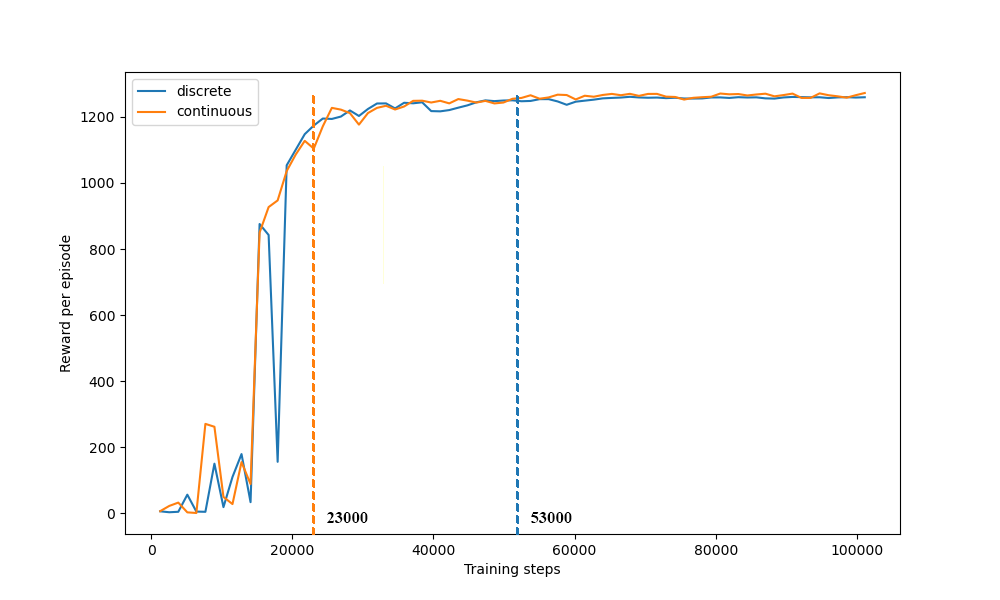
\includegraphics[width=\textwidth]{Figures/SP_discrete_vs_continuous_training_time.png}
		\label{fig: sp - training time}
		\caption{1-link system. Agent in continuous action space reaches maximum number of successful tests in approximately of 23000 timesteps.}
	\end{subfigure}
	\hfill
	\begin{subfigure}[t]{0.48\textwidth}
		\centering
		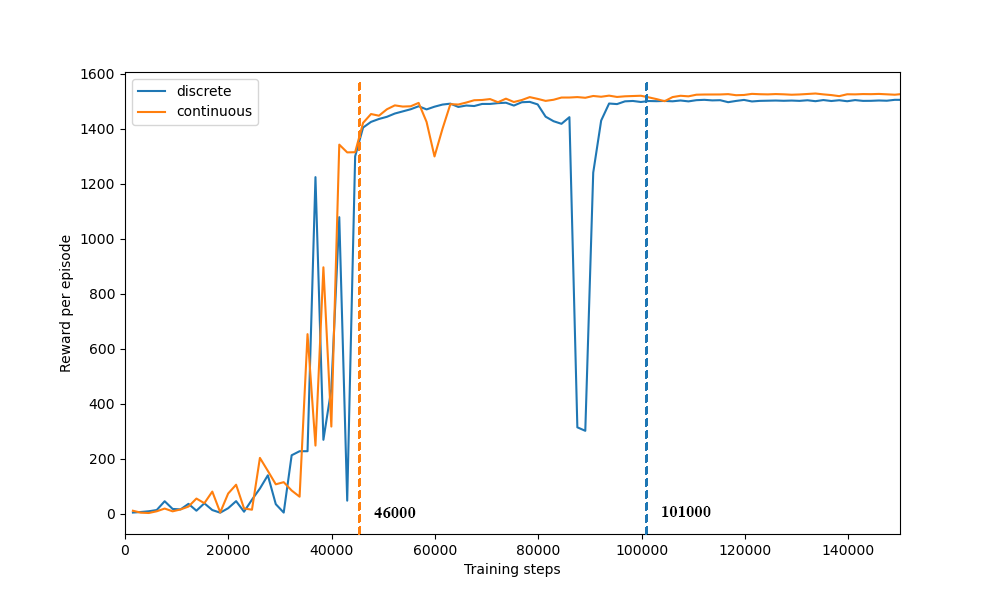
\includegraphics[width=\textwidth]{Figures/DP_discrete_vs_continuous_training_time.png}
		\label{fig: dp - training time}
		\caption{2-link system. At the timesteps of 46000 the agent has reached the maximum number of successful tests.}
	\end{subfigure}
	\begin{subfigure}[t]{0.48\textwidth}
		\centering
		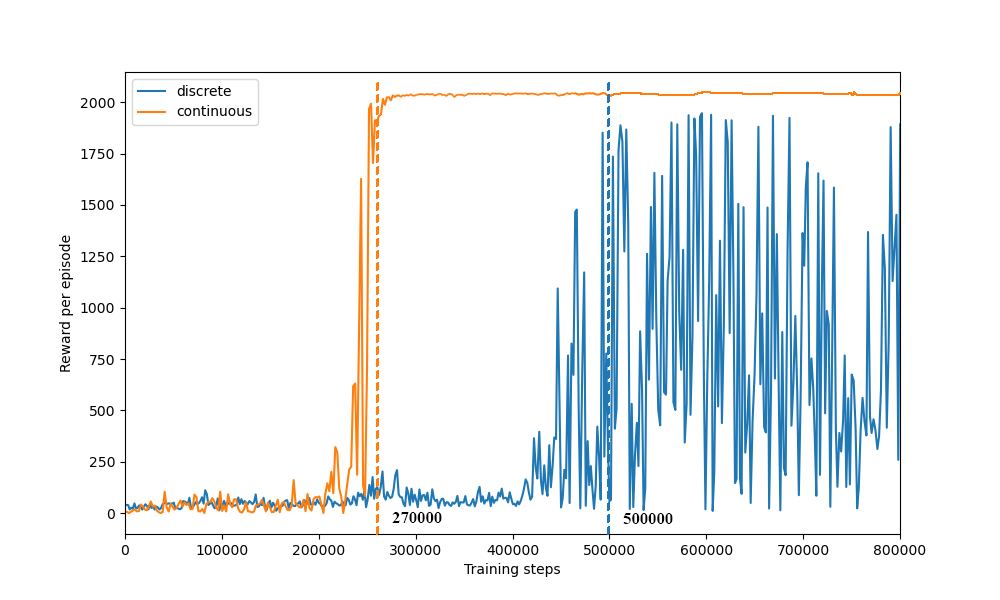
\includegraphics[width=\textwidth]{Figures/TP_discrete_vs_continuous_training_time.png}
		\label{fig: tp - training time}
		\caption{3-link system. Less then 300000 timesteps required to train the system with the usage of continuous action space.}
	\end{subfigure}
	
	\caption{Training times for the PPO agents for 1-link (a), 2-link (b) and 3-link (c) systems}
	\label{fig: training time comparison}
\end{figure}

The continuous action space consistently demonstrates superior stability across all systems, as reflected in the smoother reward curves after convergence. It also reduces training time on up to 50\% for an agent to achieve a maximum number of successful tests. In contrast, the discrete action space leads to more oscillatory performance, particularly in more complex systems, which could indicate less efficient exploration and exploitation during training.

For a deeper evaluation of the continuous control scheme in comparison to the discrete one, we have created a stability zone, the development of which is described in our work of Manzl et al.~\cite{manzl2023relrl}. From an engineering standpoint, not only are the randomized tests used for evaluation important, but it is also crucial to identify an area where the agent successfully performs the stabilization task for practical, real-world applications. The stability zones are shown in Figure~\ref{fig: continuous vs discrete} and illustrate the performance of discrete (orange) and continuous (light yellow) action spaces. These zones represent the regions in state space where the agent successfully maintains the pendulum's stability. The axes represent different state variables depending on the system's complexity, as detailed below.
For the 1-link system (Figure~\ref{fig: continuous vs discrete} (a)) the stability zones are depicted as elongated regions around the origin where the pendulum is successfully balanced. X-axis represent the link's angle and Y-axis its angular velocity. The continuous action space encompasses a slightly broader area compared to the discrete action space, indicating a greater tolerance for variations in the angle and angular velocity. This suggests that the continuous action space provides more flexibility in controlling the pendulum, allowing it to stabilize from a wider range of initial conditions. For the 2-link system (Figure~\ref{fig: continuous vs discrete} (b)), the stability zones are narrower and more elongated, reflecting the increased complexity of the system. First and the second link angle combinations are presented in this zone. The continuous action space again covers a slightly larger area than the discrete action space, particularly along the axis. This expanded zone suggests that the continuous action space better handles the interactions between the two links, allowing for more robust stabilization strategies. In the 3-link system (Figure~\ref{fig: continuous vs discrete} (c) and Figure~\ref{fig: continuous vs discrete} (d)), the stability zones become even more restricted, particularly in the second plot, where the angles of the second and third links are plotted. The continuous action space consistently outperforms the discrete space by maintaining a larger stability region in both plots. The narrower orange zones indicate that the discrete action space struggles with the additional degrees of freedom, whereas the continuous action space adapts more effectively to the system's increased complexity.

\begin{figure}[h!]
	\centering
	\begin{subfigure}[t]{0.48\textwidth}
		\centering
		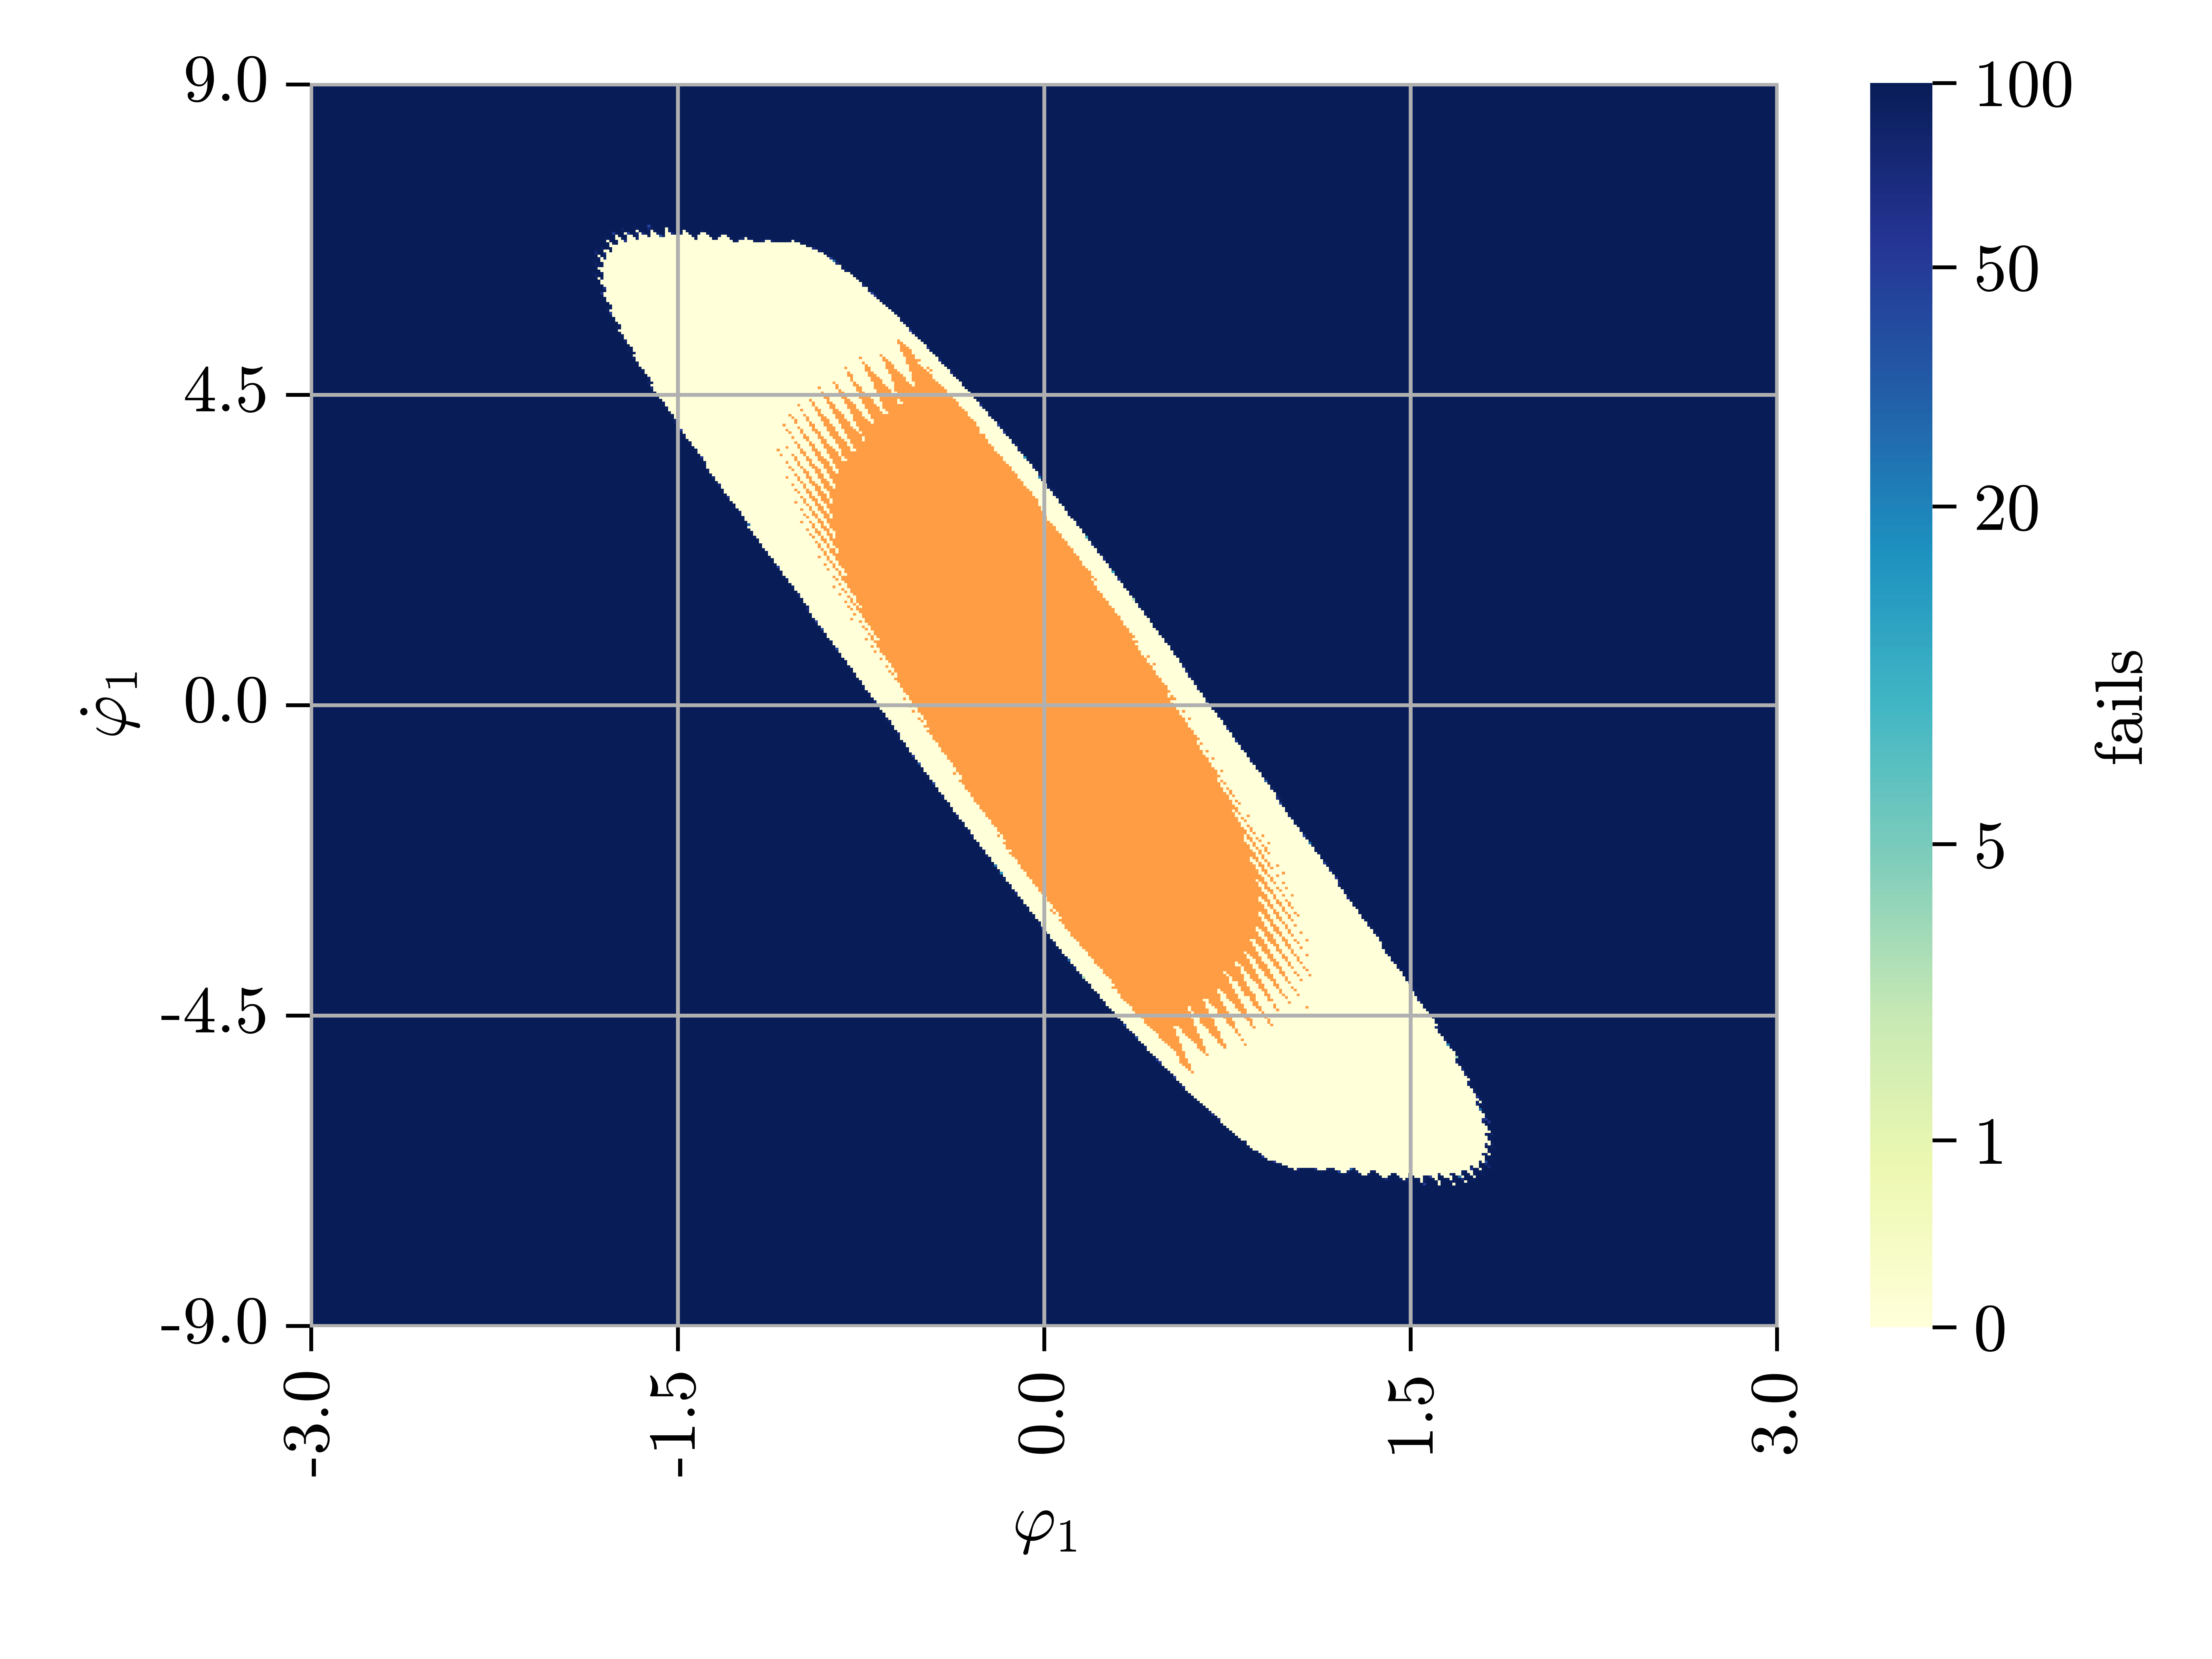
\includegraphics[width=\textwidth]{Figures/SP_continuous_vs_discrete_phi1phi1dot.png}
		\label{fig: sp - continuous vs discrete}
		\caption{}
	\end{subfigure}
	\hfill
	\begin{subfigure}[t]{0.48\textwidth}
		\centering
		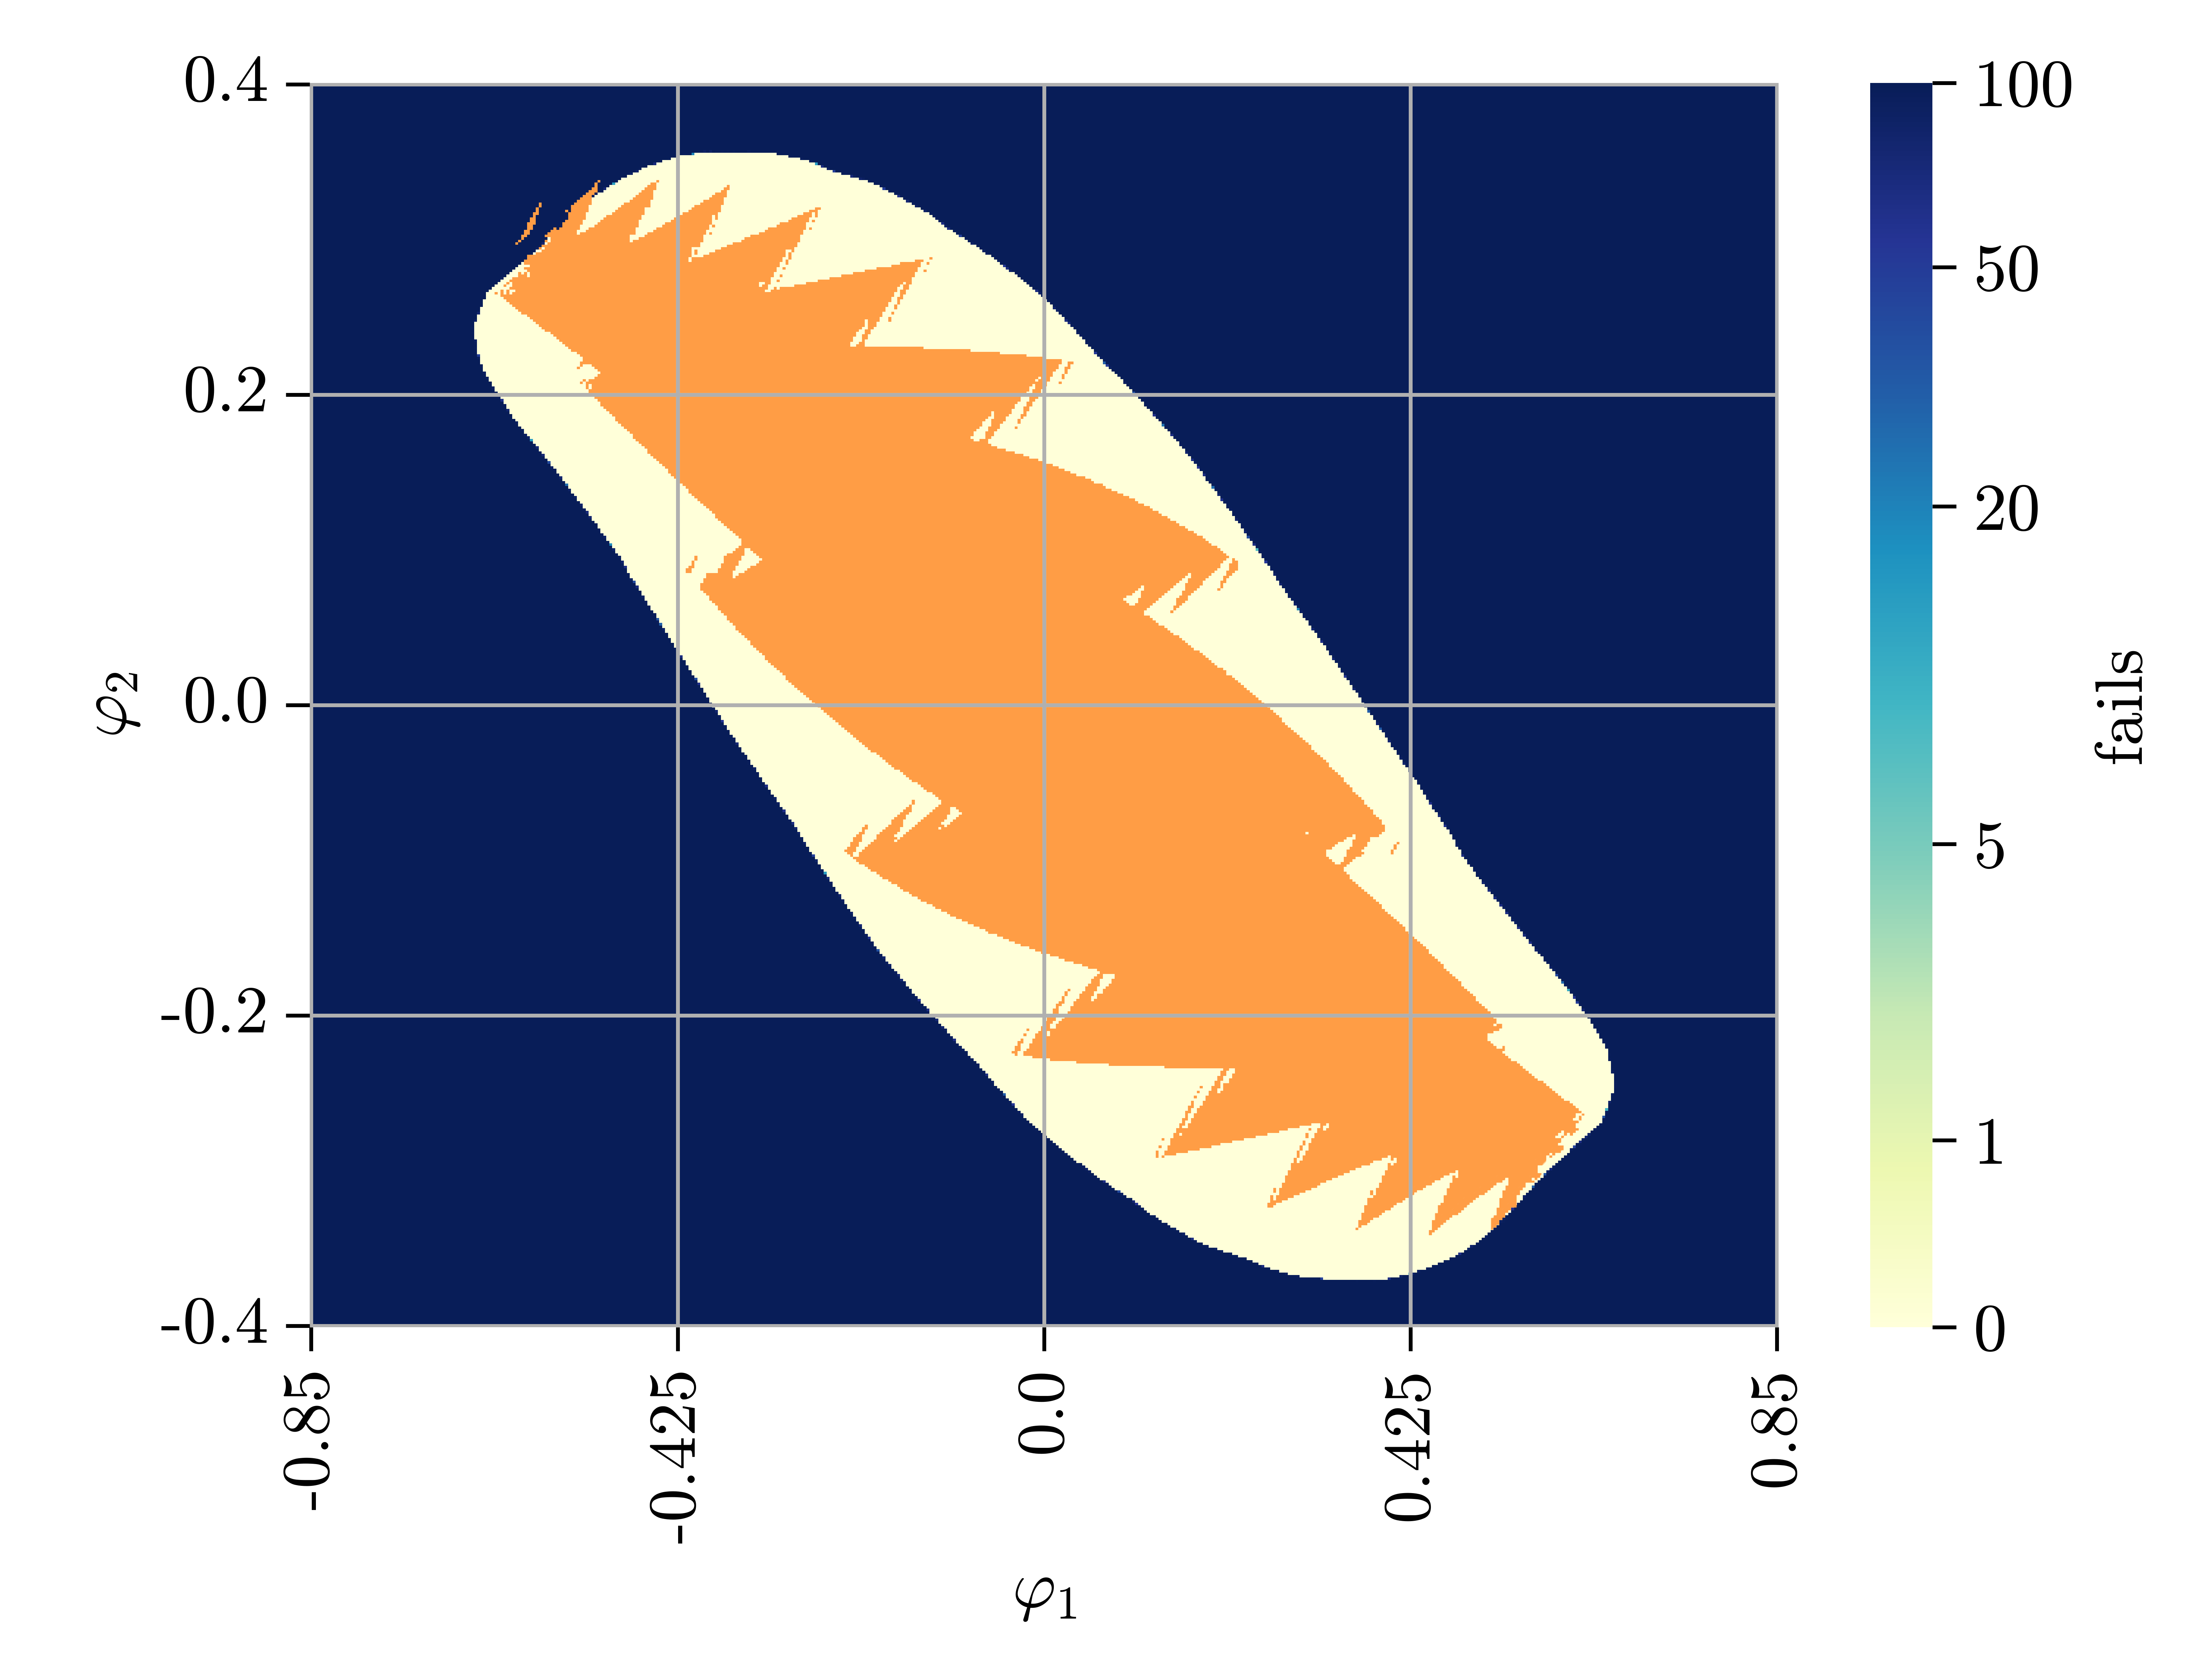
\includegraphics[width=\textwidth]{Figures/DP_continuous_vs_discrete_phi1phi2.png}
		\label{fig: dp - continuous vs discrete}
		\caption{}
	\end{subfigure}
	
	\vspace{0.2cm}
	
	\begin{subfigure}[t]{0.48\textwidth}
		\centering
		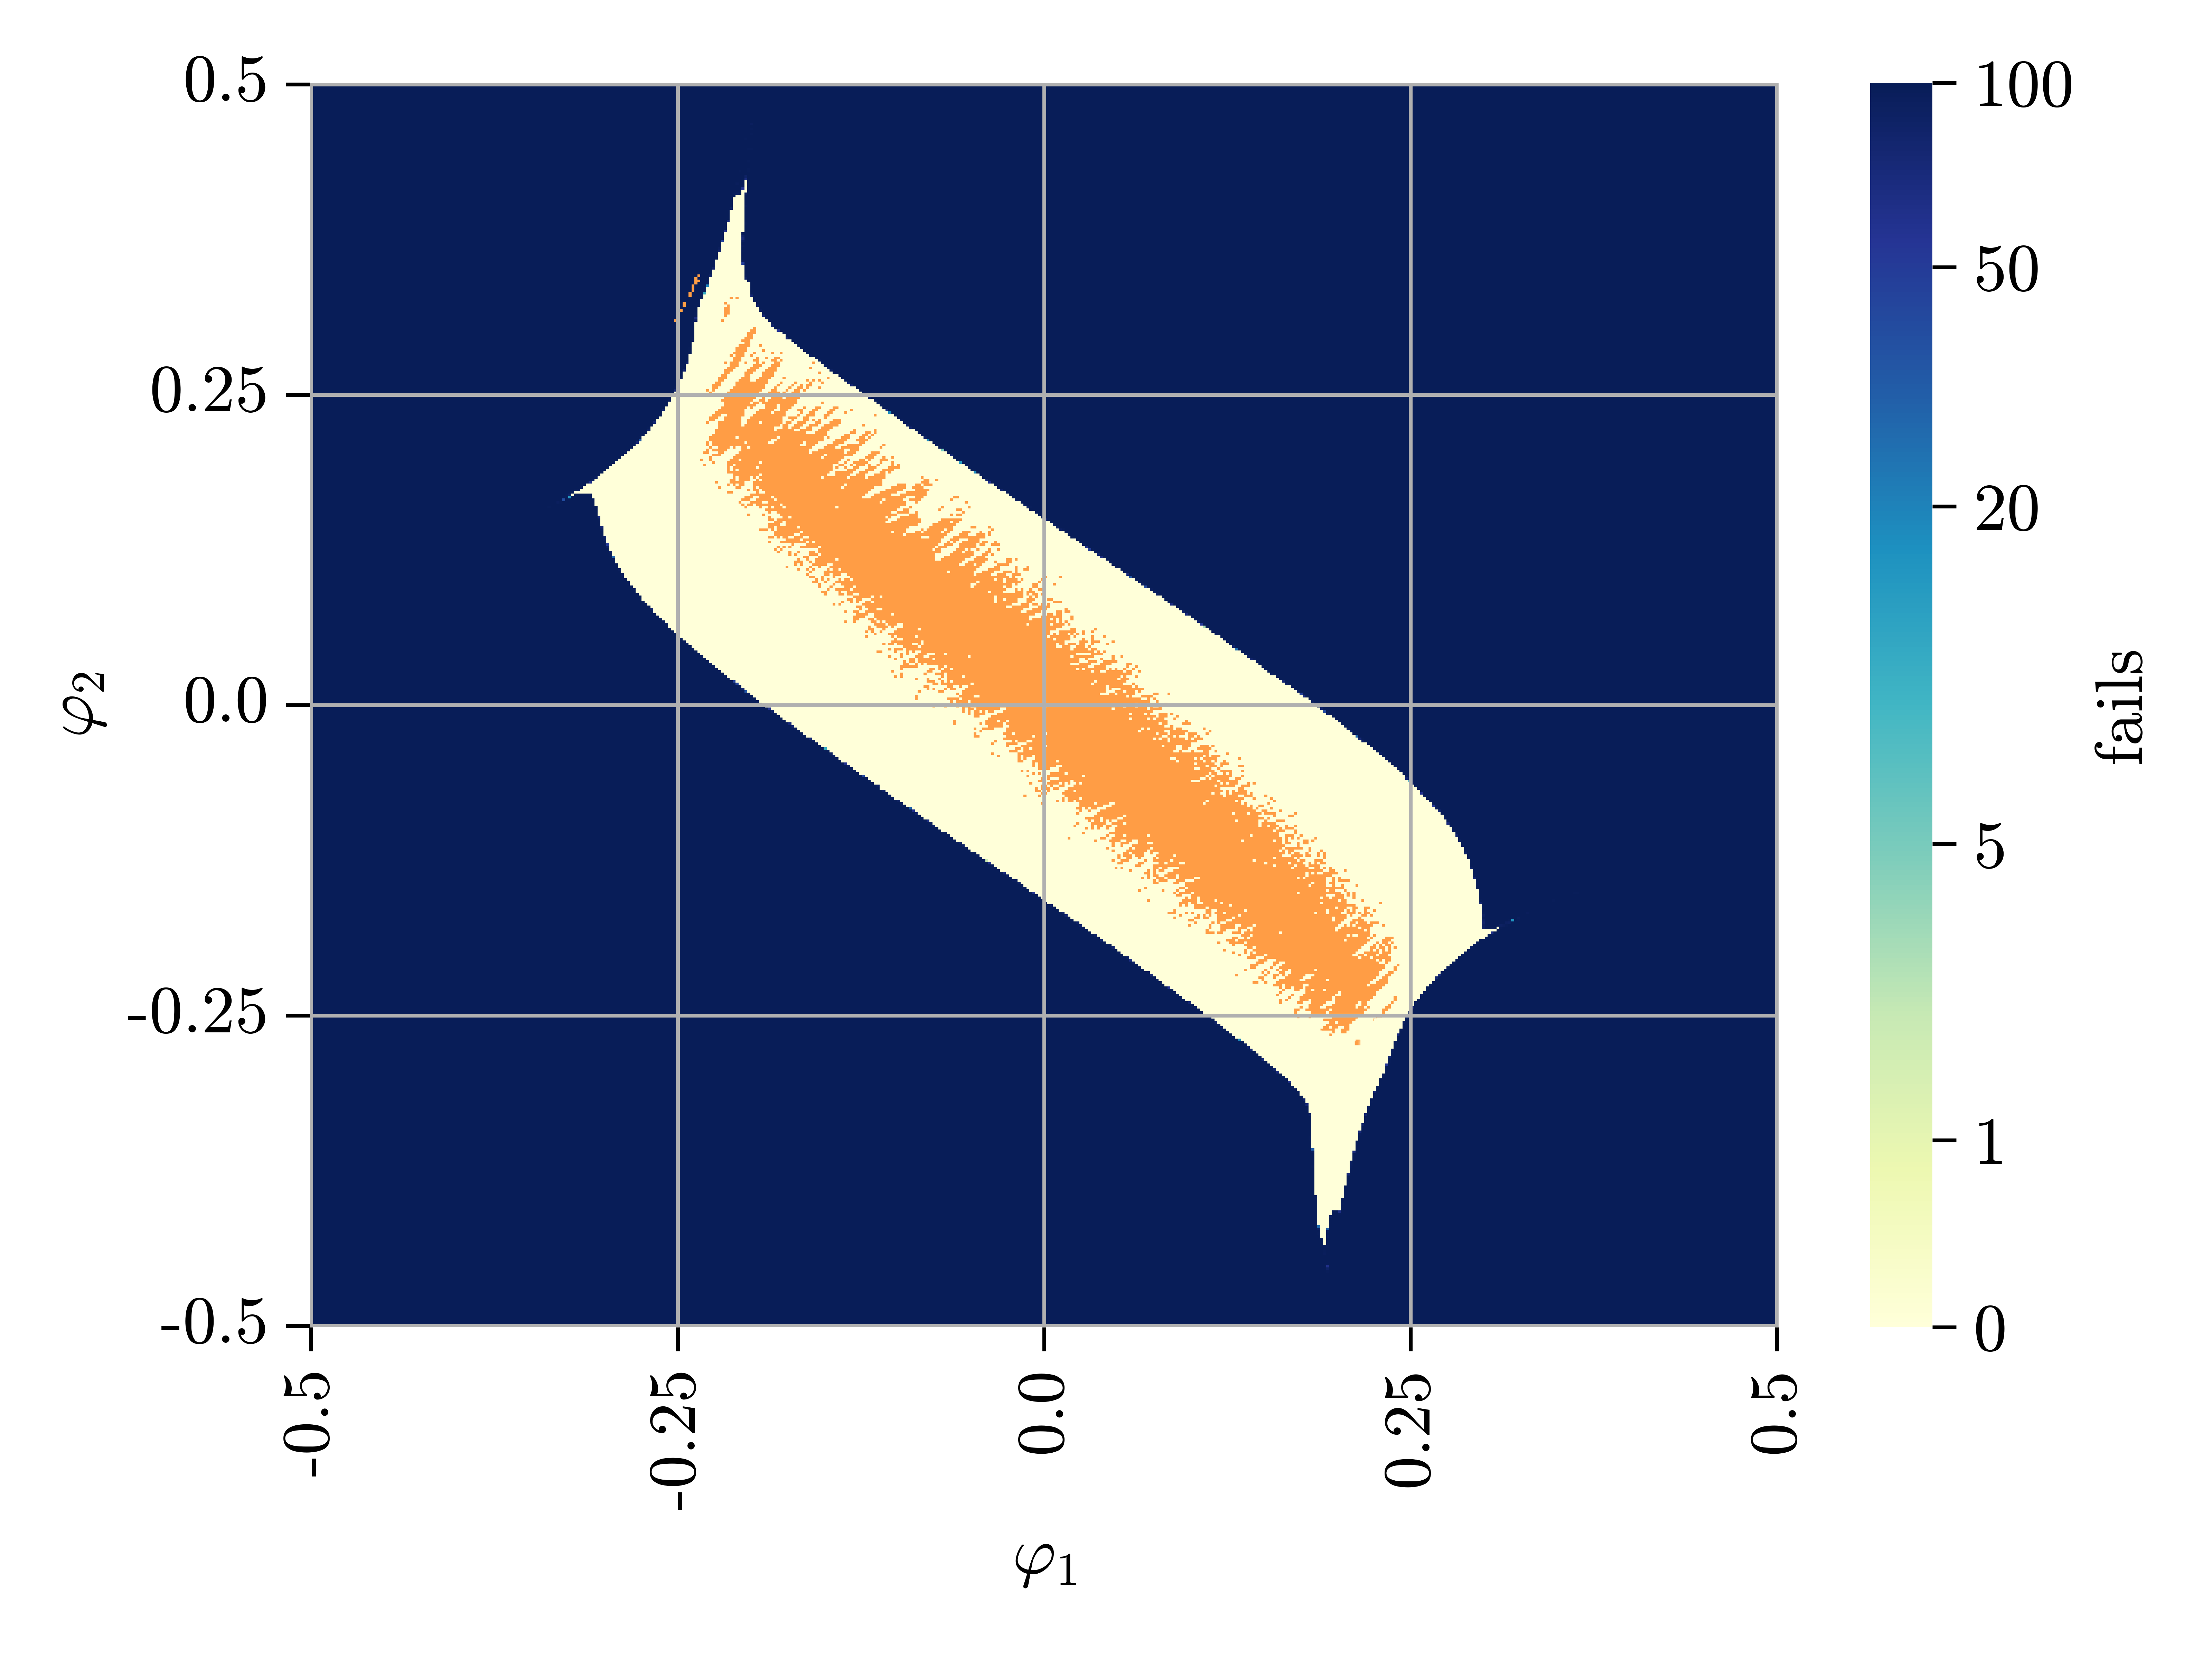
\includegraphics[width=\textwidth]{Figures/TP_continuous_vs_discrete_phi1phi2.png}
		\label{fig: tp - continuous vs discrete, phi1 phi2}
		\caption{}
	\end{subfigure}
	\hfill
	\begin{subfigure}[t]{0.48\textwidth}
		\centering
		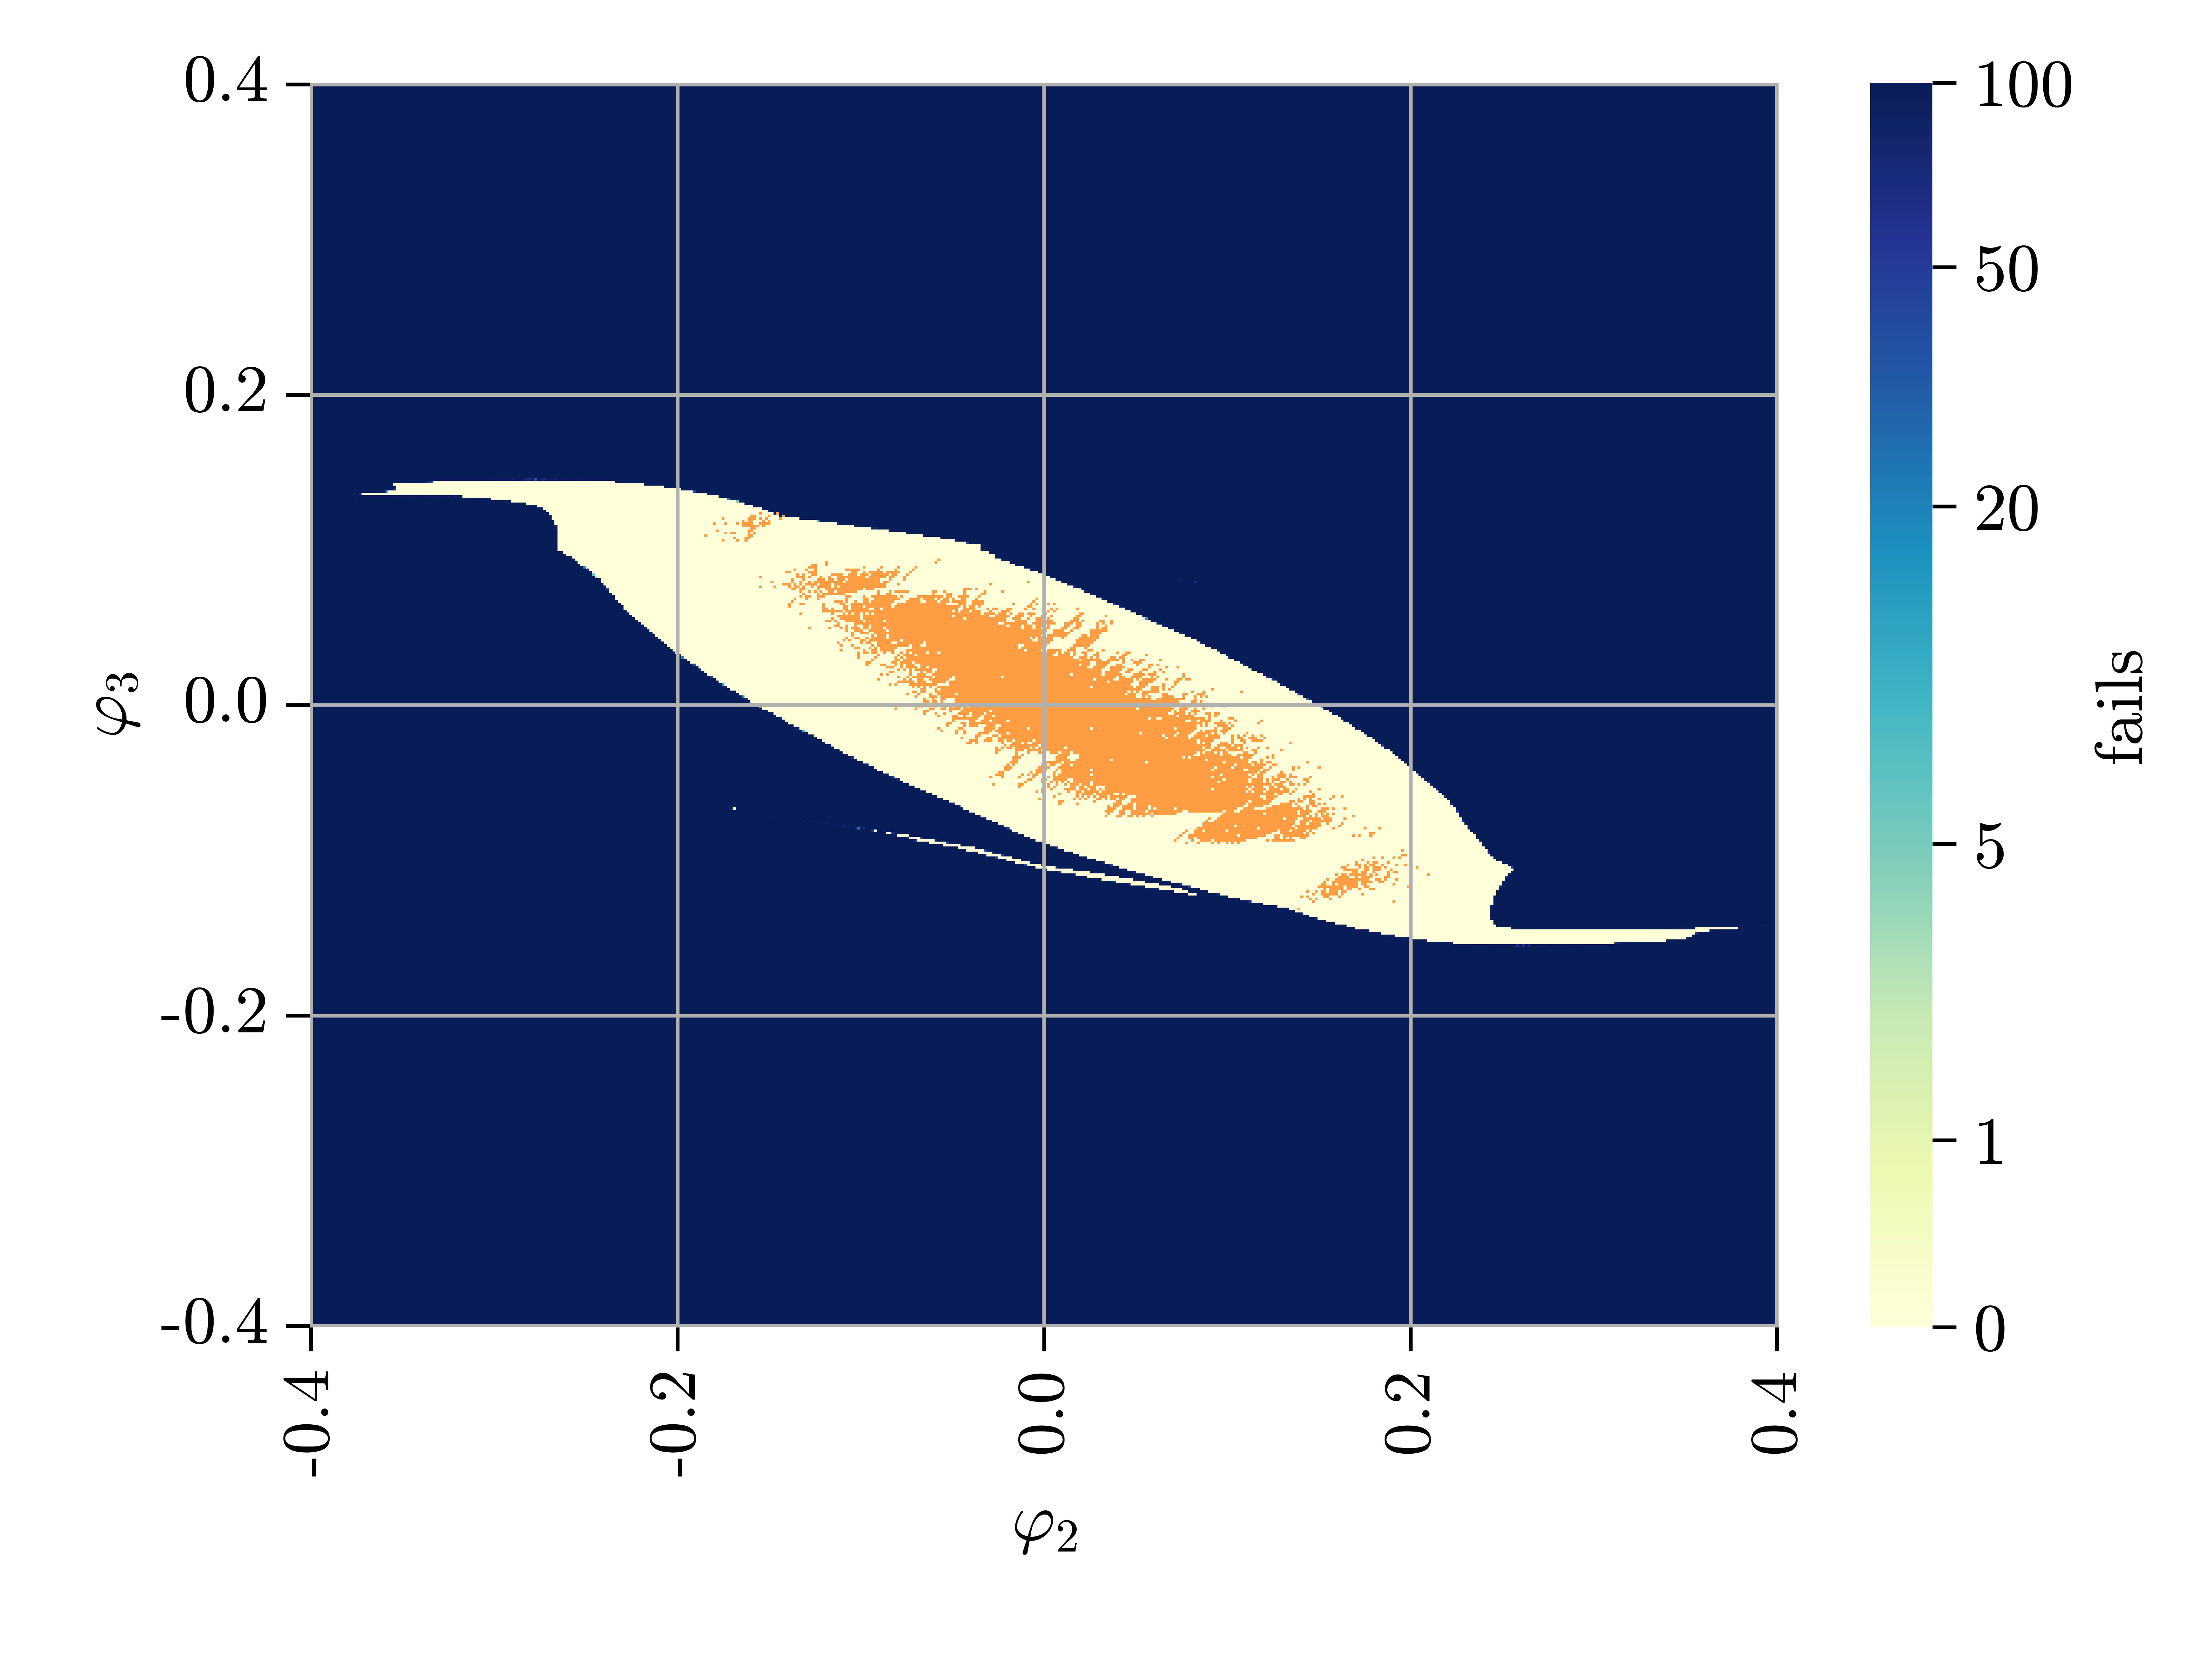
\includegraphics[width=\textwidth]{Figures/TP_continuous_vs_discrete_phi2phi3.png}
		\label{fig: tp - continuous vs discrete, phi2 phi3}
		\caption{}
	\end{subfigure}
	
	\caption{Stability zones comparison of the PPO agent using different control strategies. For the 1-link system (a) the zone axis are link's angle $\phi_1$ and angular velocity $\dot{\phi_1}$, while for the 2-link system (b) axis are the pendulum link angles $\phi_1$ and $\phi_2$. Figures (b) and (c) present the stability zones based on the dependence of pendulum link angles of $\phi_1$ and $\phi_2$ and of $\phi_2$ and $\phi_3$. The discrete control stability zone is indicated in orange; continuous is in white beige. Each grid cell represents 100 randomized tests.}
	\label{fig: continuous vs discrete}
\end{figure}

These stability zones highlight the advantages of continuous action spaces in maintaining the stability of multi-link inverted pendulum systems. As the system's complexity increases (from 1-link to 3-link), the continuous action space's broader stability regions suggest a higher robustness to variations in state variables, making it more effective in stabilizing complex systems.
The continuous action space's ability to control a wider range of initial conditions is particularly beneficial in systems with multiple degrees of freedom, where precise and adaptive control strategies are required. This is evident in the progressively more complex systems, where the continuous action space maintains larger stability zones, indicating better overall performance.
These findings support the notion that continuous action spaces may be more suitable for applications requiring fine-tuned control in high-dimensional environments, where the ability to handle a broader range of state variations is crucial for success.

\subsection{Agents with continuous action space tested on modified environments} \label{subsec: Agent tested on modified environments}

In this section, we examine the impact of changing properties of the environment, namely
link length, mass, and added friction, on the stability zones. The friction is implemented in the same fashion as in our previous study~\cite{manzl2023relrl} and is modeled using Coulomb friction, characterized by a friction torque, which opposes rotation and is independent of the applied forces. The investigation is conducted
using the inverted double pendulum on a cart model (same continuous agent as in the Figure~\ref{fig: continuous vs discrete} (b)). In each subplot of Figure~\ref{fig: agent impact on different environments}, the stability zone is determined for the same agent in various modified environments, and the contour of the stability zone from the original environment is overlaid.

 \begin{figure}[h!]
     \centering
     \begin{subfigure}[t]{0.32\textwidth}
         \centering
         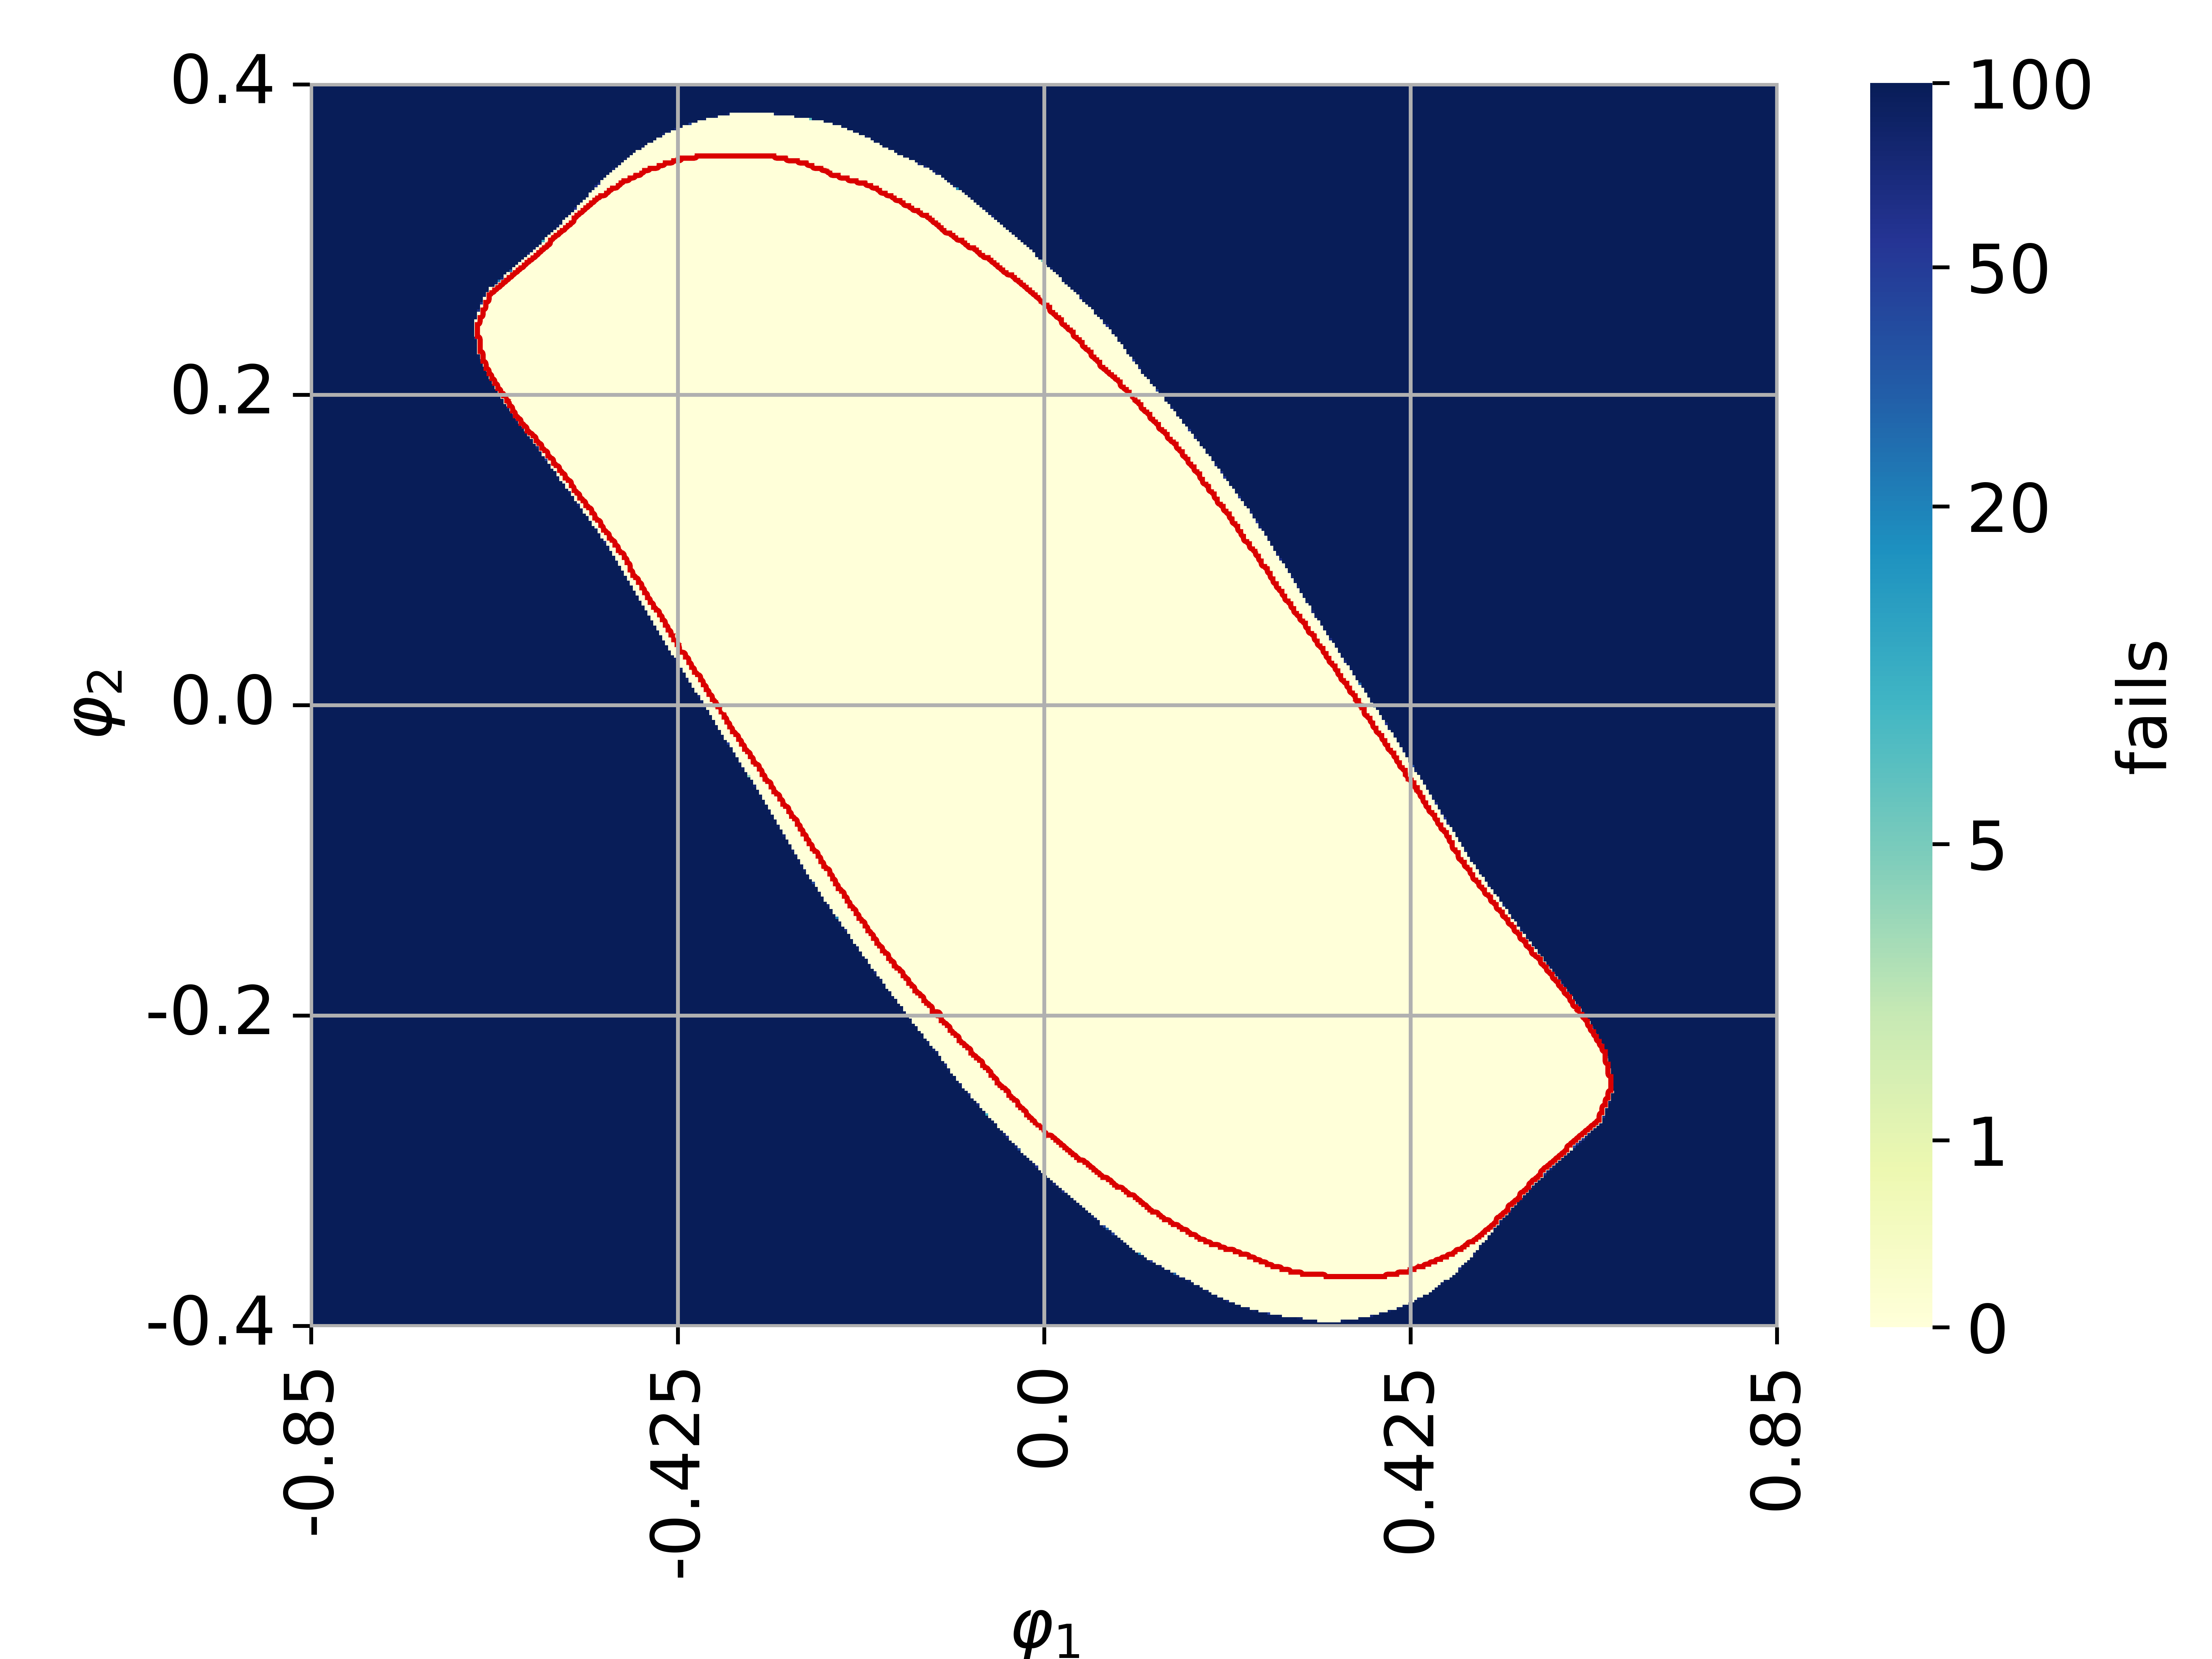
\includegraphics[width=\textwidth]{Figures/DP_len_1.1.png}
         \label{fig: DP len 1.1}
         \caption{}
     \end{subfigure}
     \hfill
     \begin{subfigure}[t]{0.32\textwidth}
         \centering
         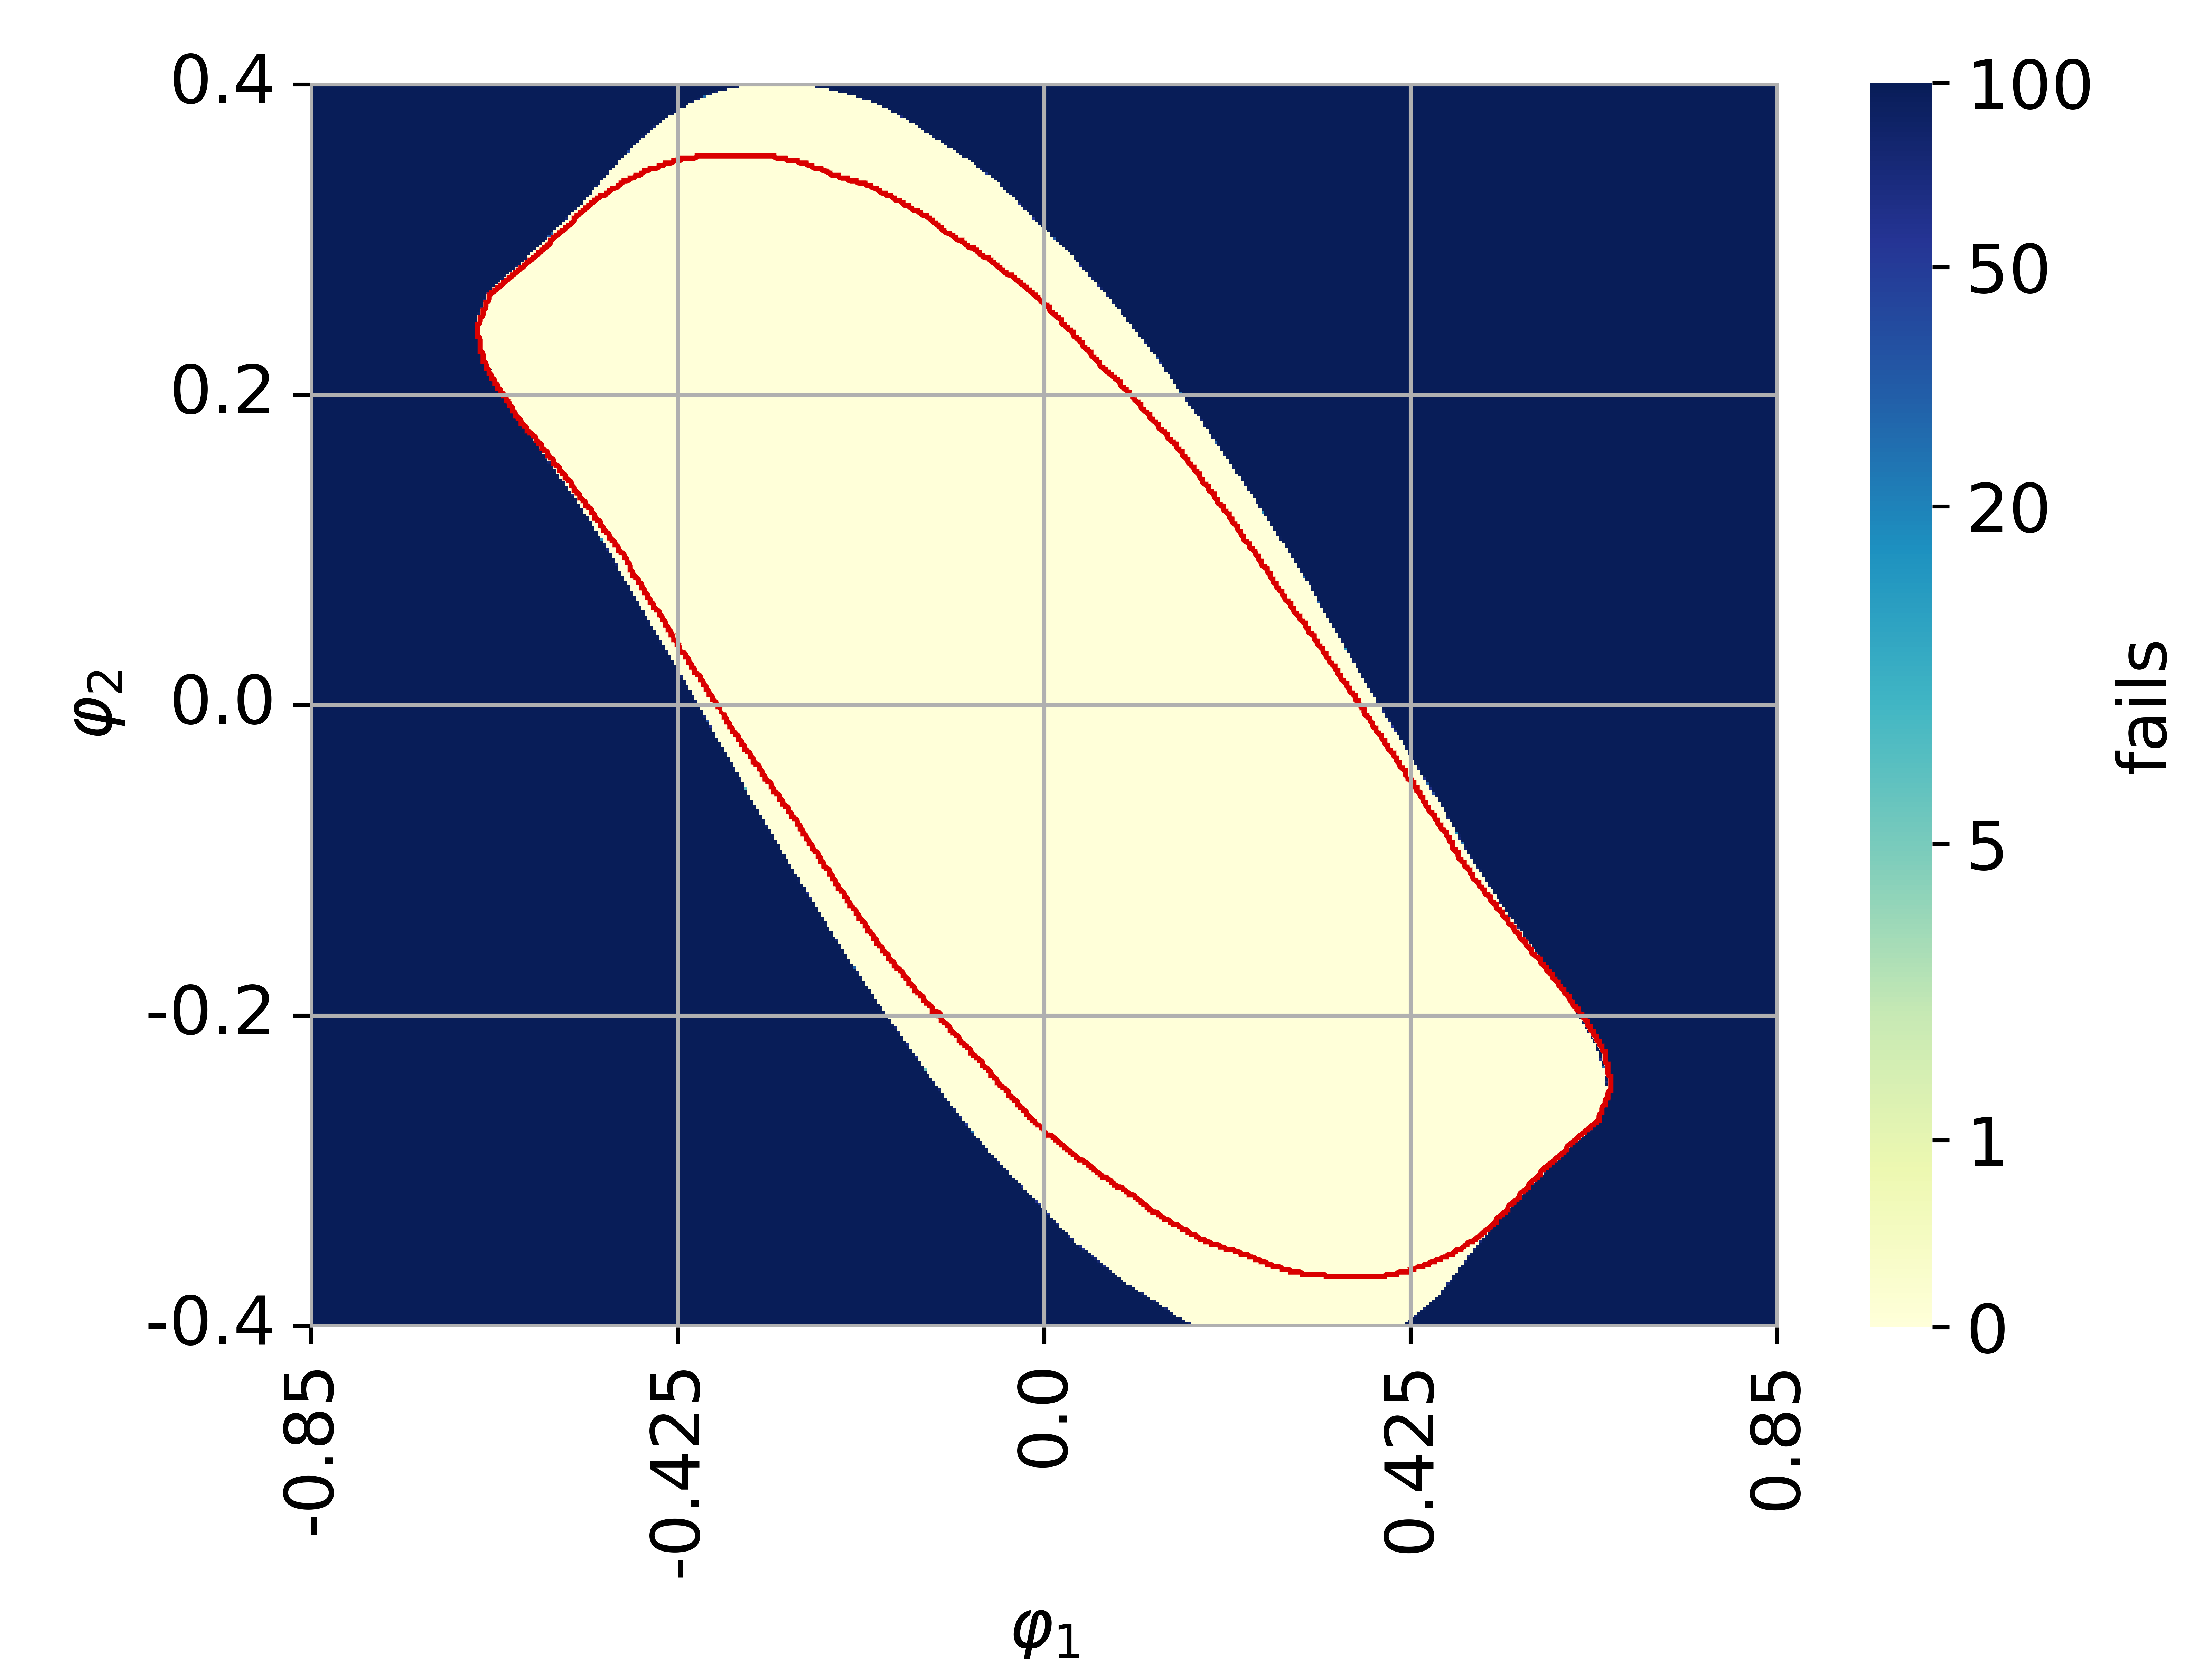
\includegraphics[width=\textwidth]{Figures/DP_len_1.2.png}
         \label{fig: DP len 1.2}
         \caption{}
     \end{subfigure}
     \hfill
     \begin{subfigure}[t]{0.32\textwidth}
         \centering
         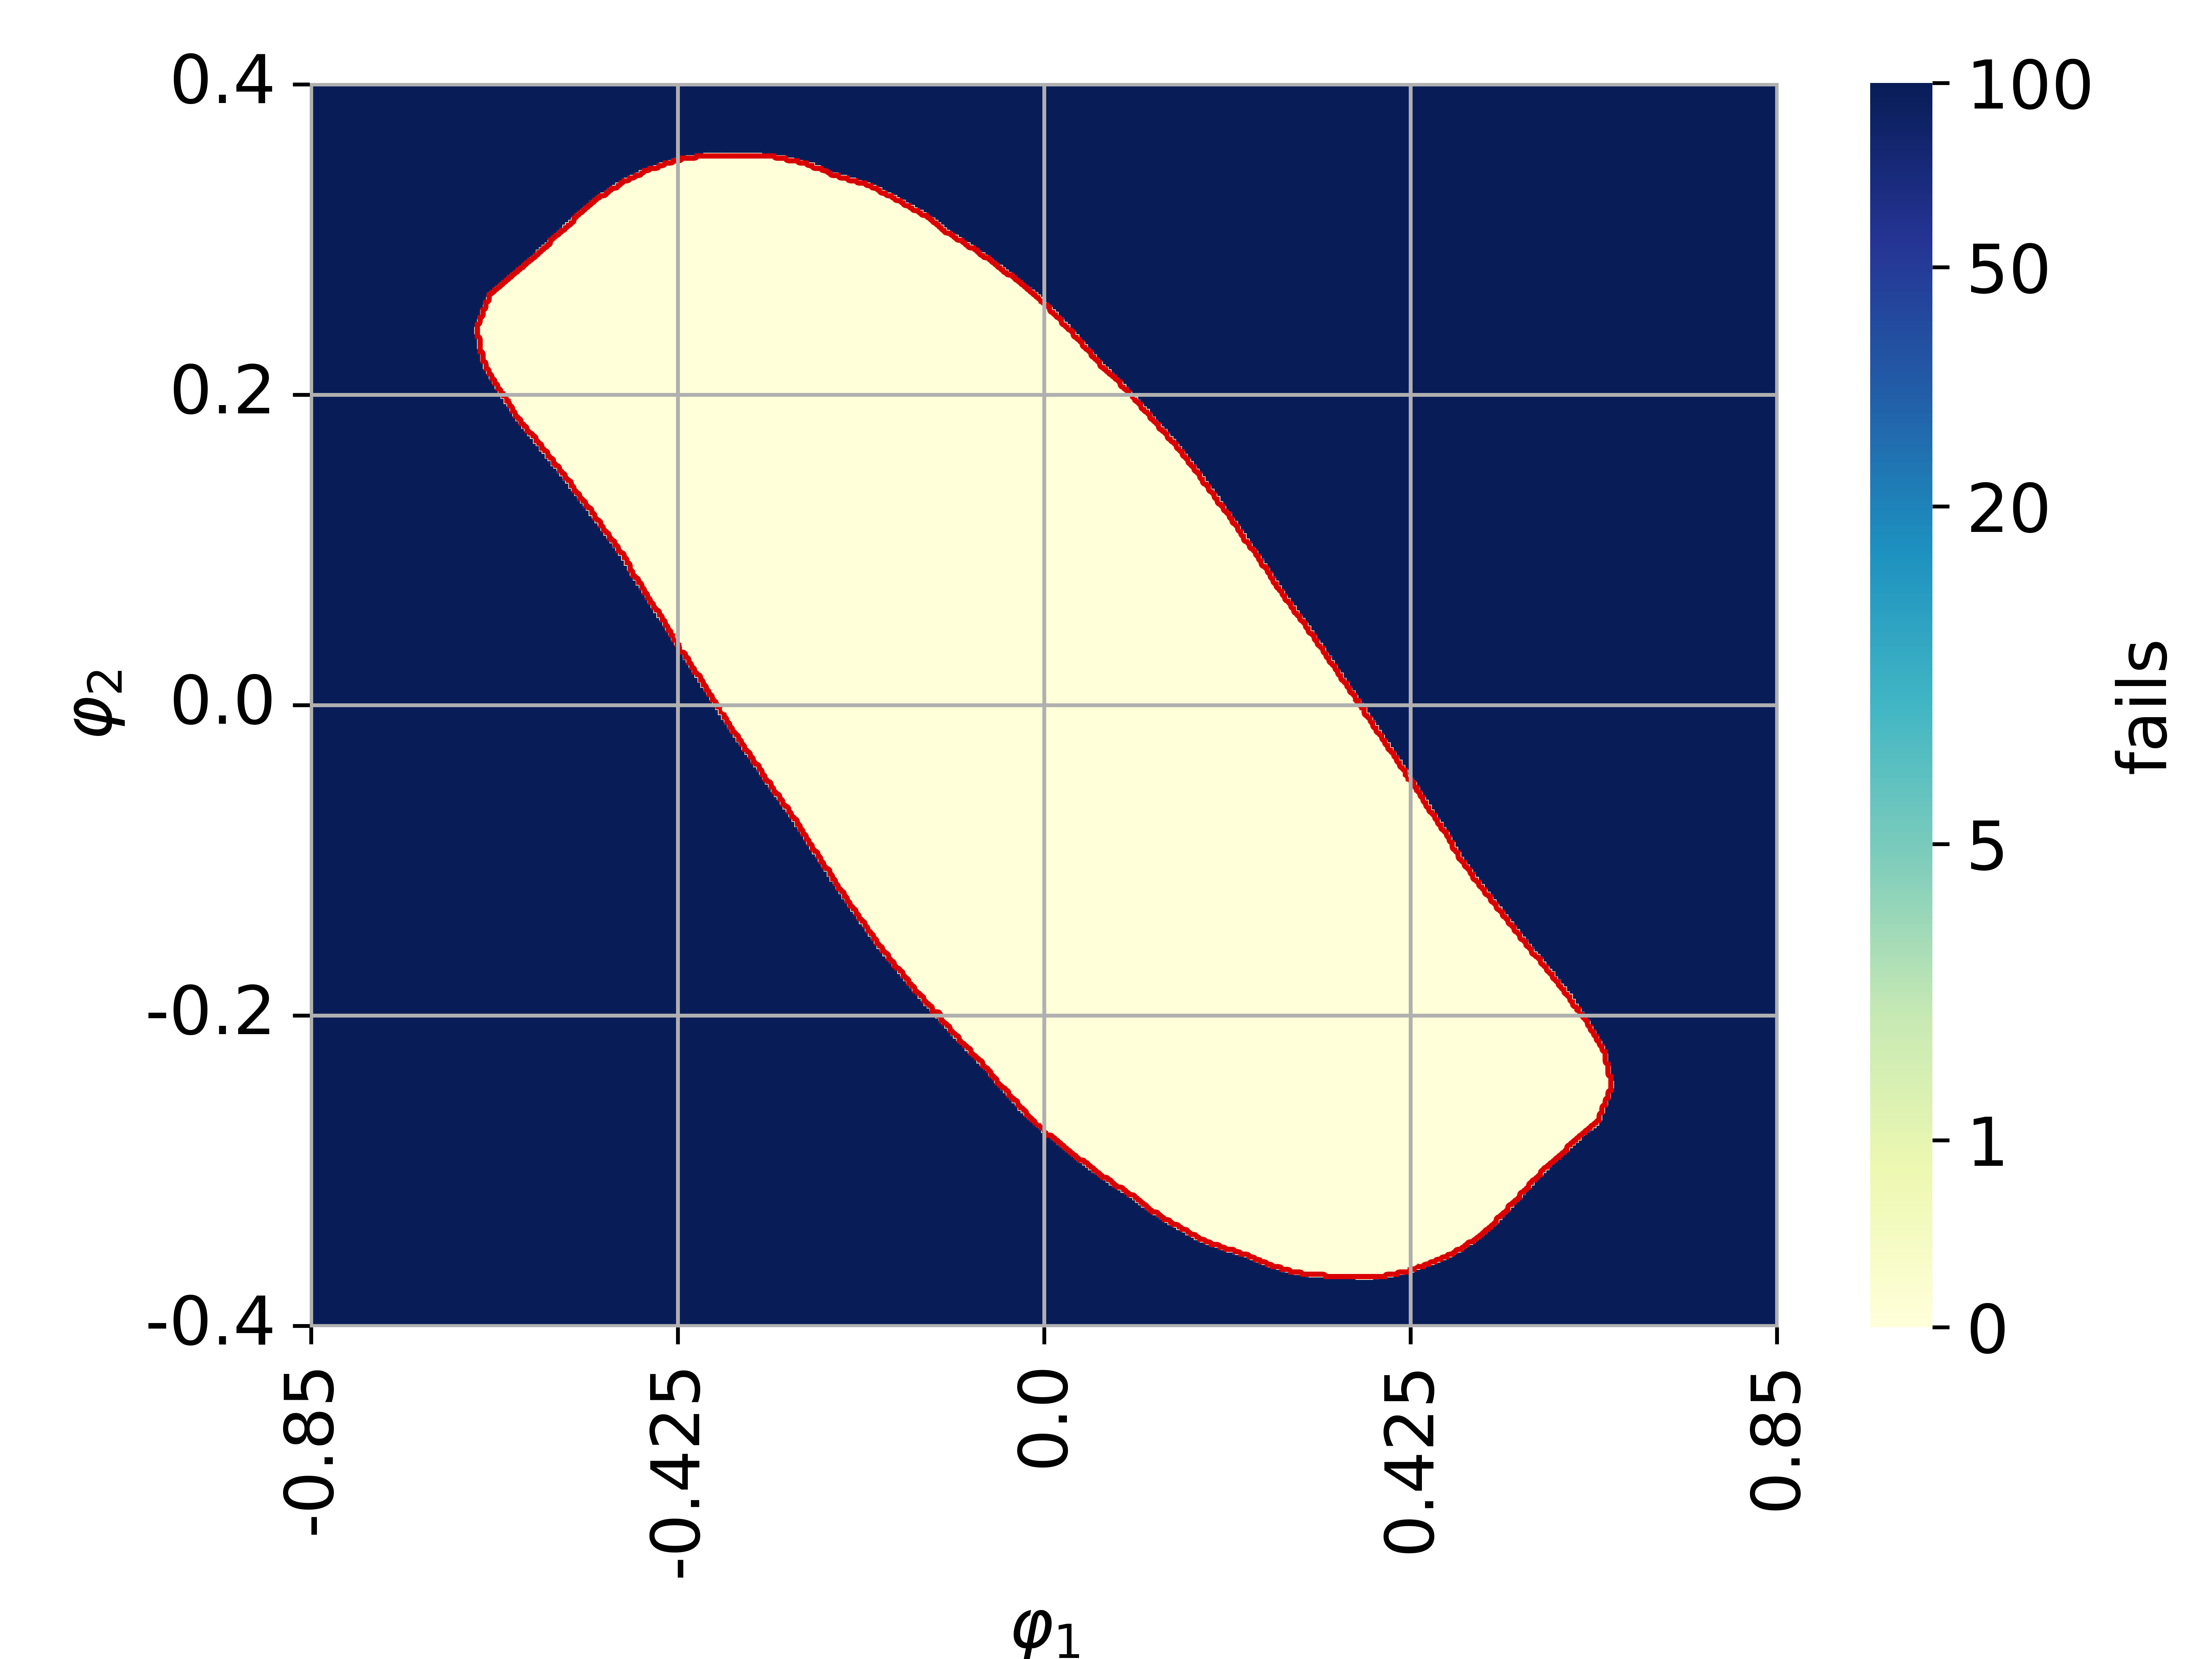
\includegraphics[width=\textwidth]{Figures/DP_mass_1.1.png}
         \label{fig: DP mass 1.1}
         \caption{}
     \end{subfigure}

     \vspace{0.2cm}

     \begin{subfigure}[t]{0.32\textwidth}
         \centering
         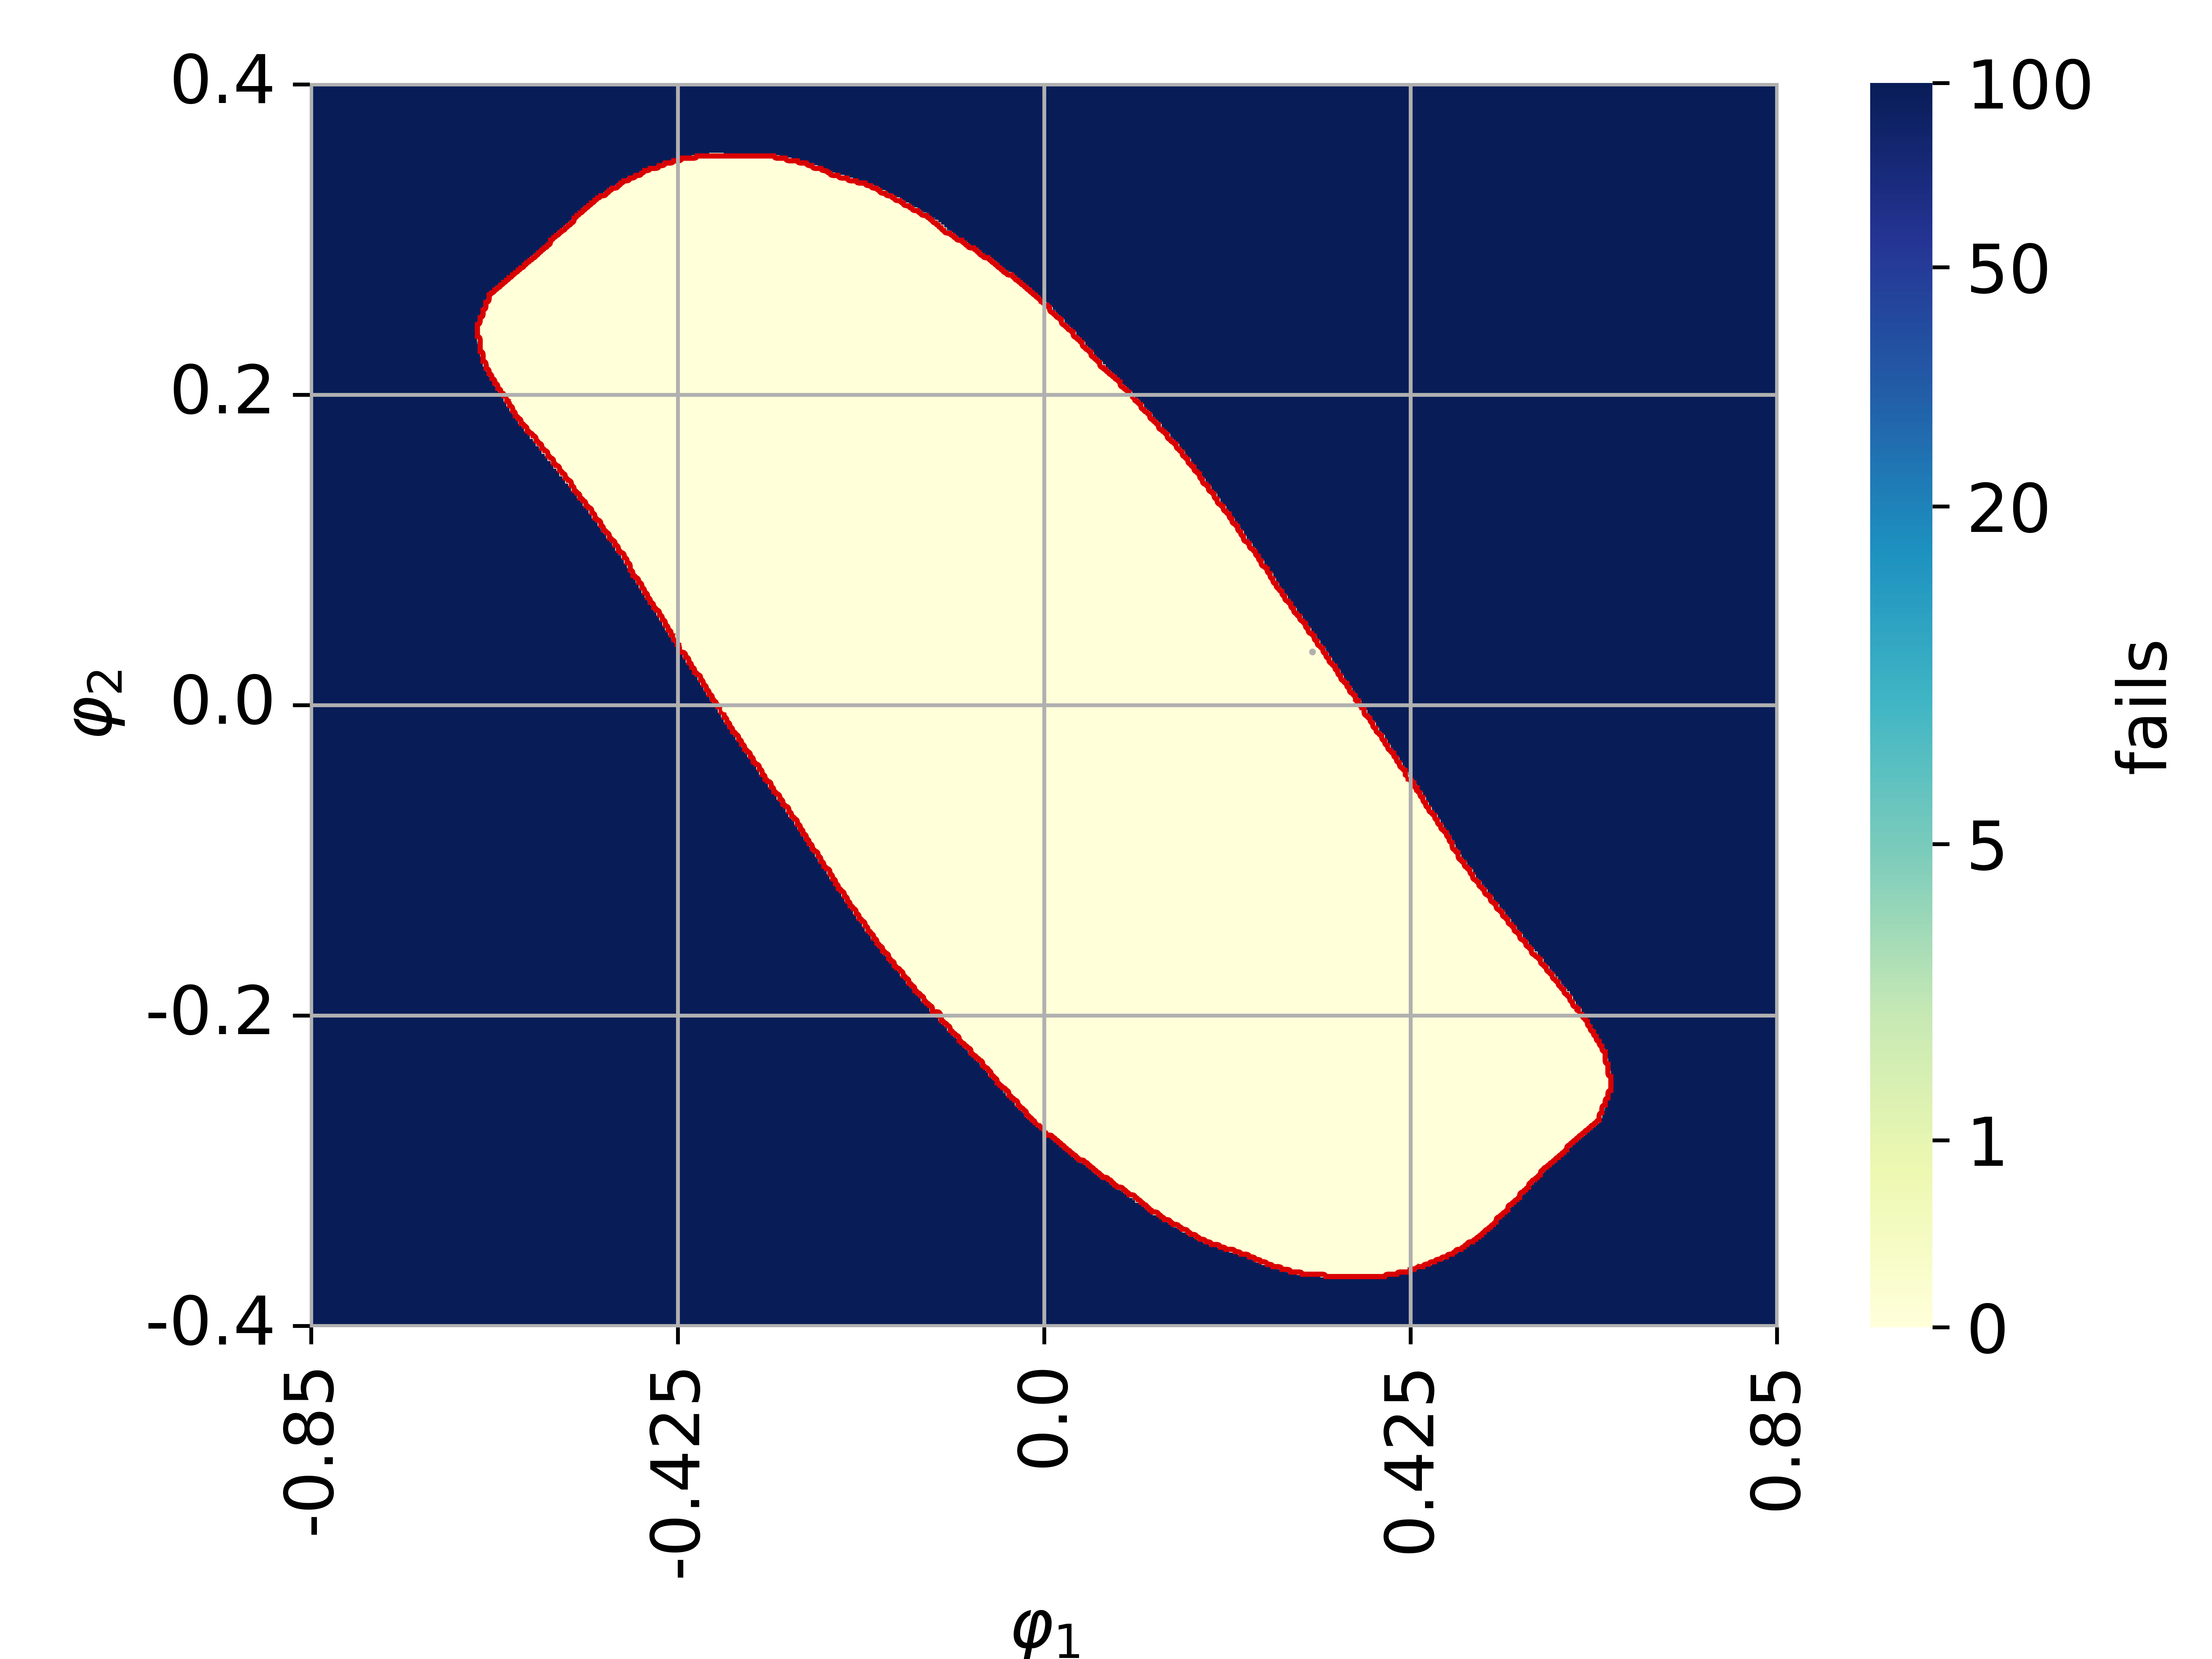
\includegraphics[width=\textwidth]{Figures/DP_mass_1.2.png}
         \label{fig: DP mass 1.2}
         \caption{}
     \end{subfigure}
     \hfill
     \begin{subfigure}[t]{0.32\textwidth}
         \centering
         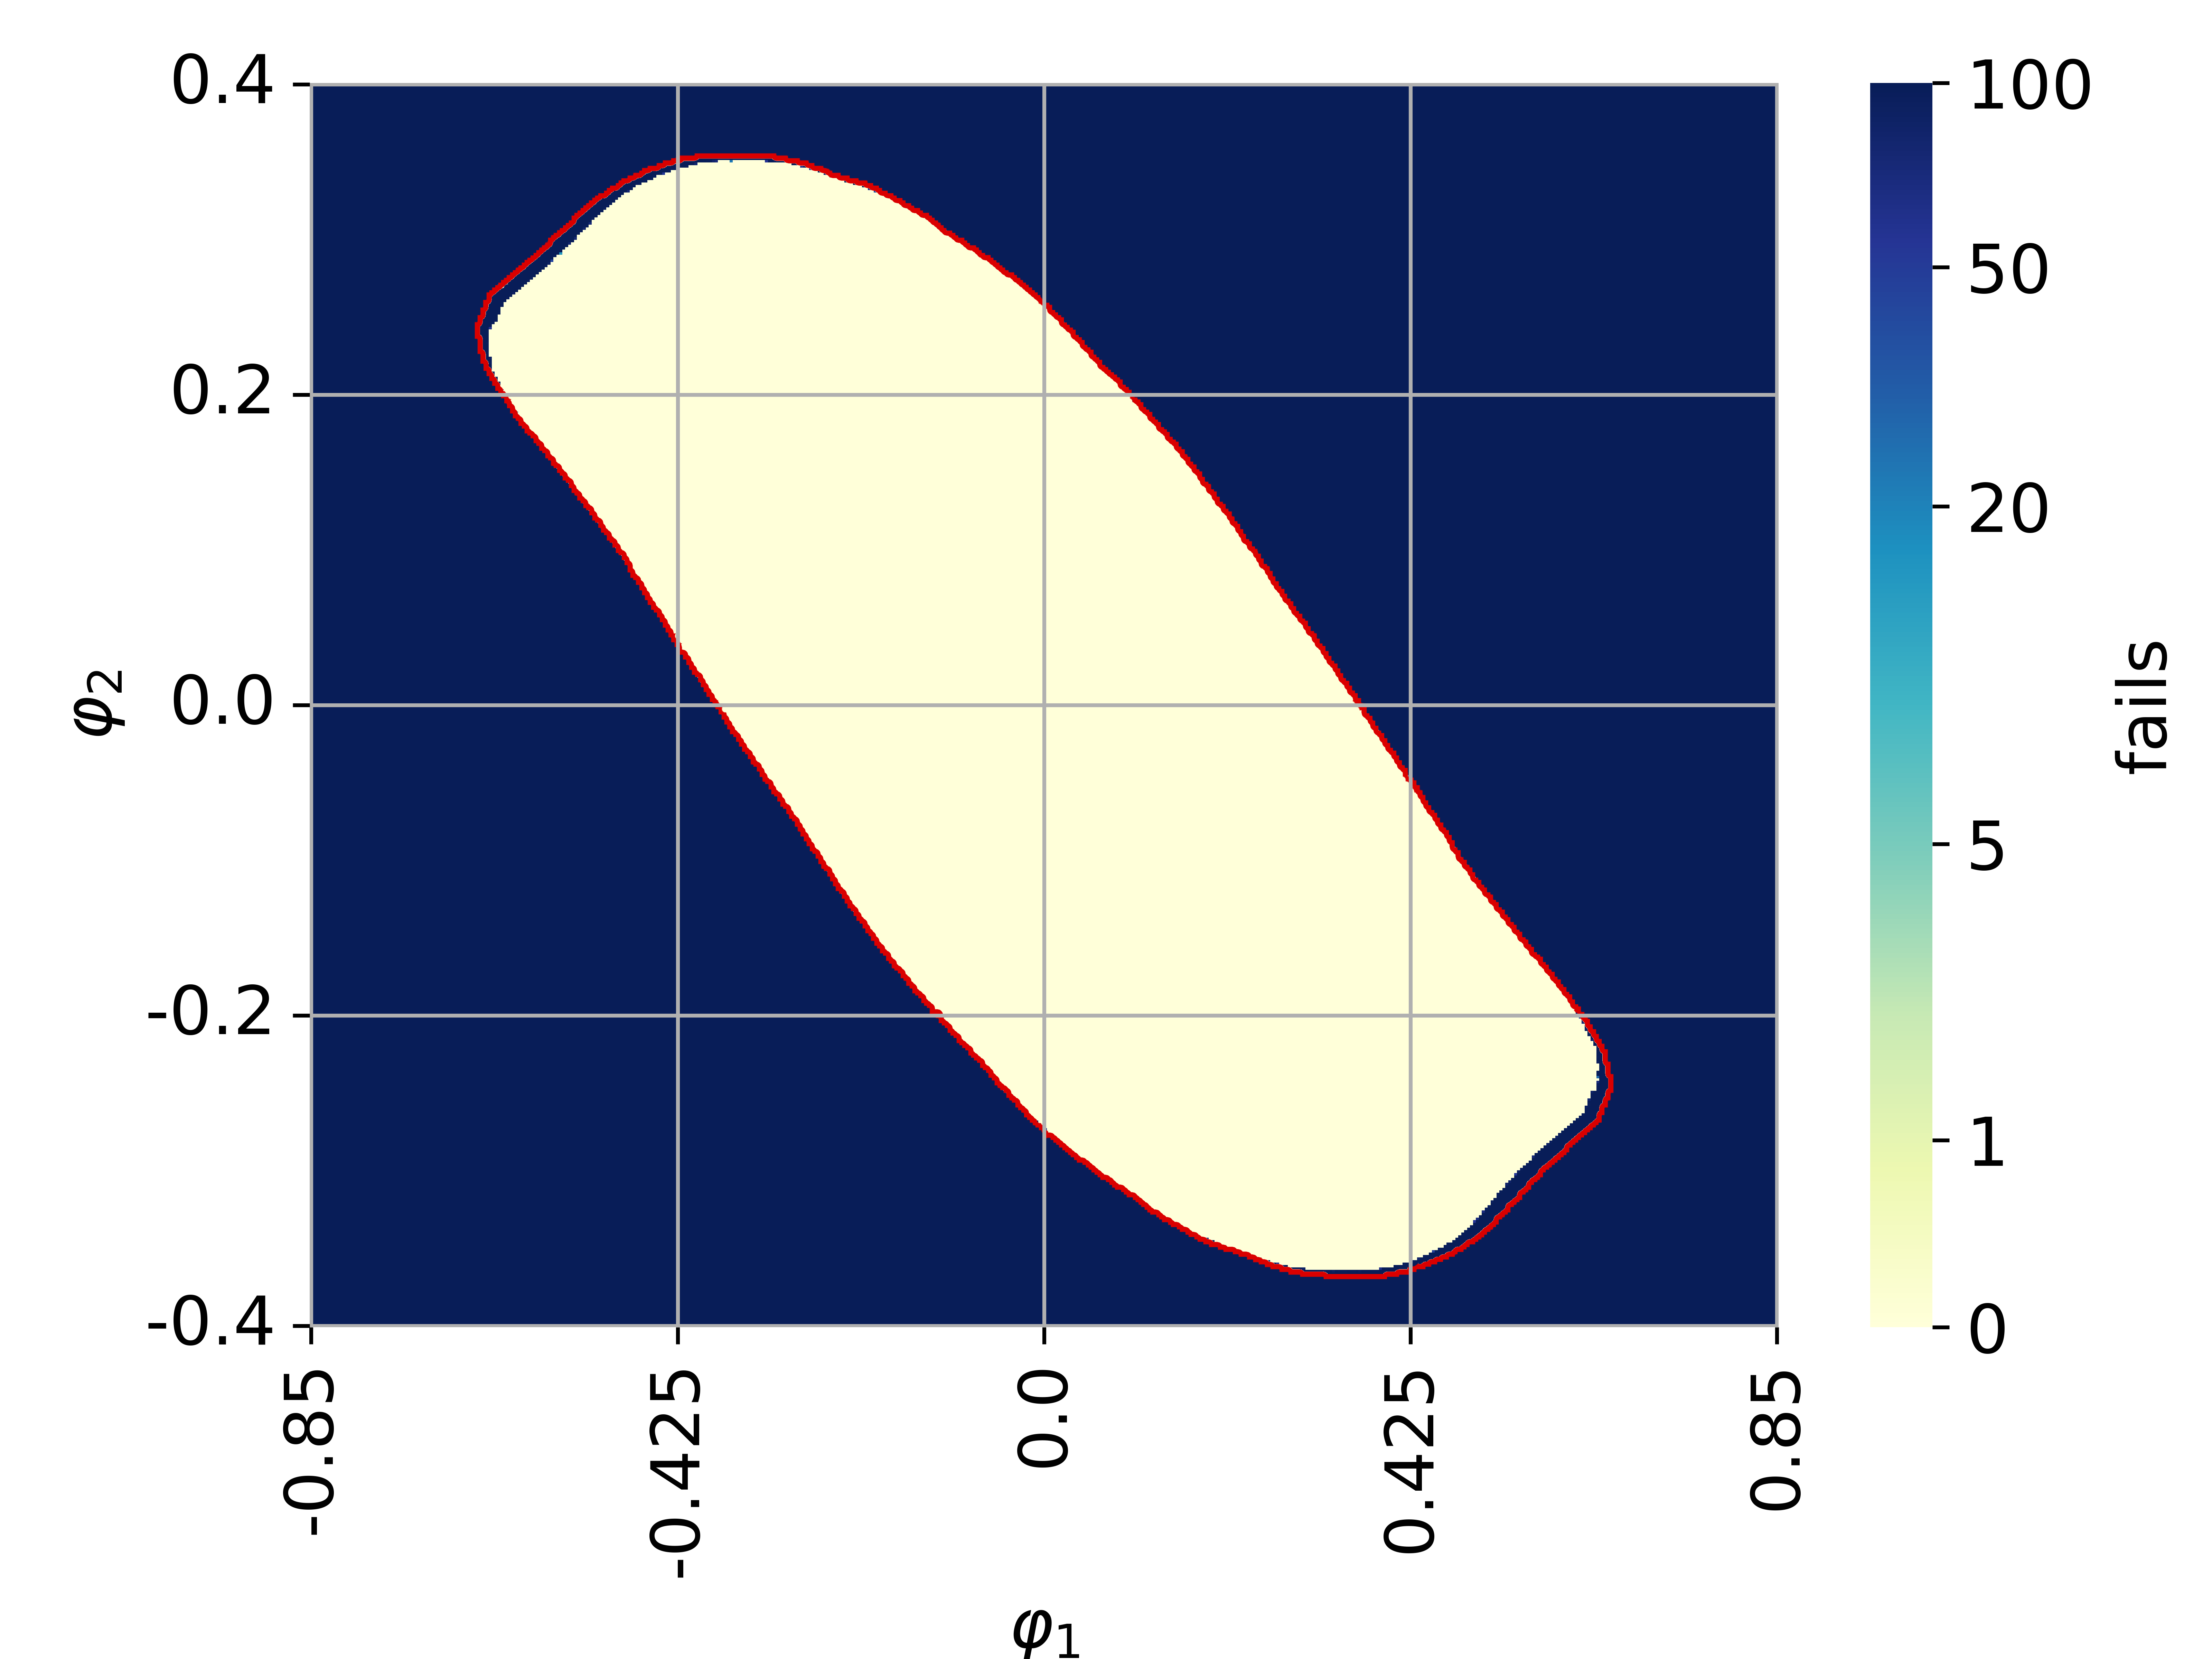
\includegraphics[width=\textwidth]{Figures/DP_friction_0.01.png}
         \label{fig: DP friction 0.01}
         \caption{}
     \end{subfigure}
     \hfill
     \begin{subfigure}[t]{0.32\textwidth}
         \centering
         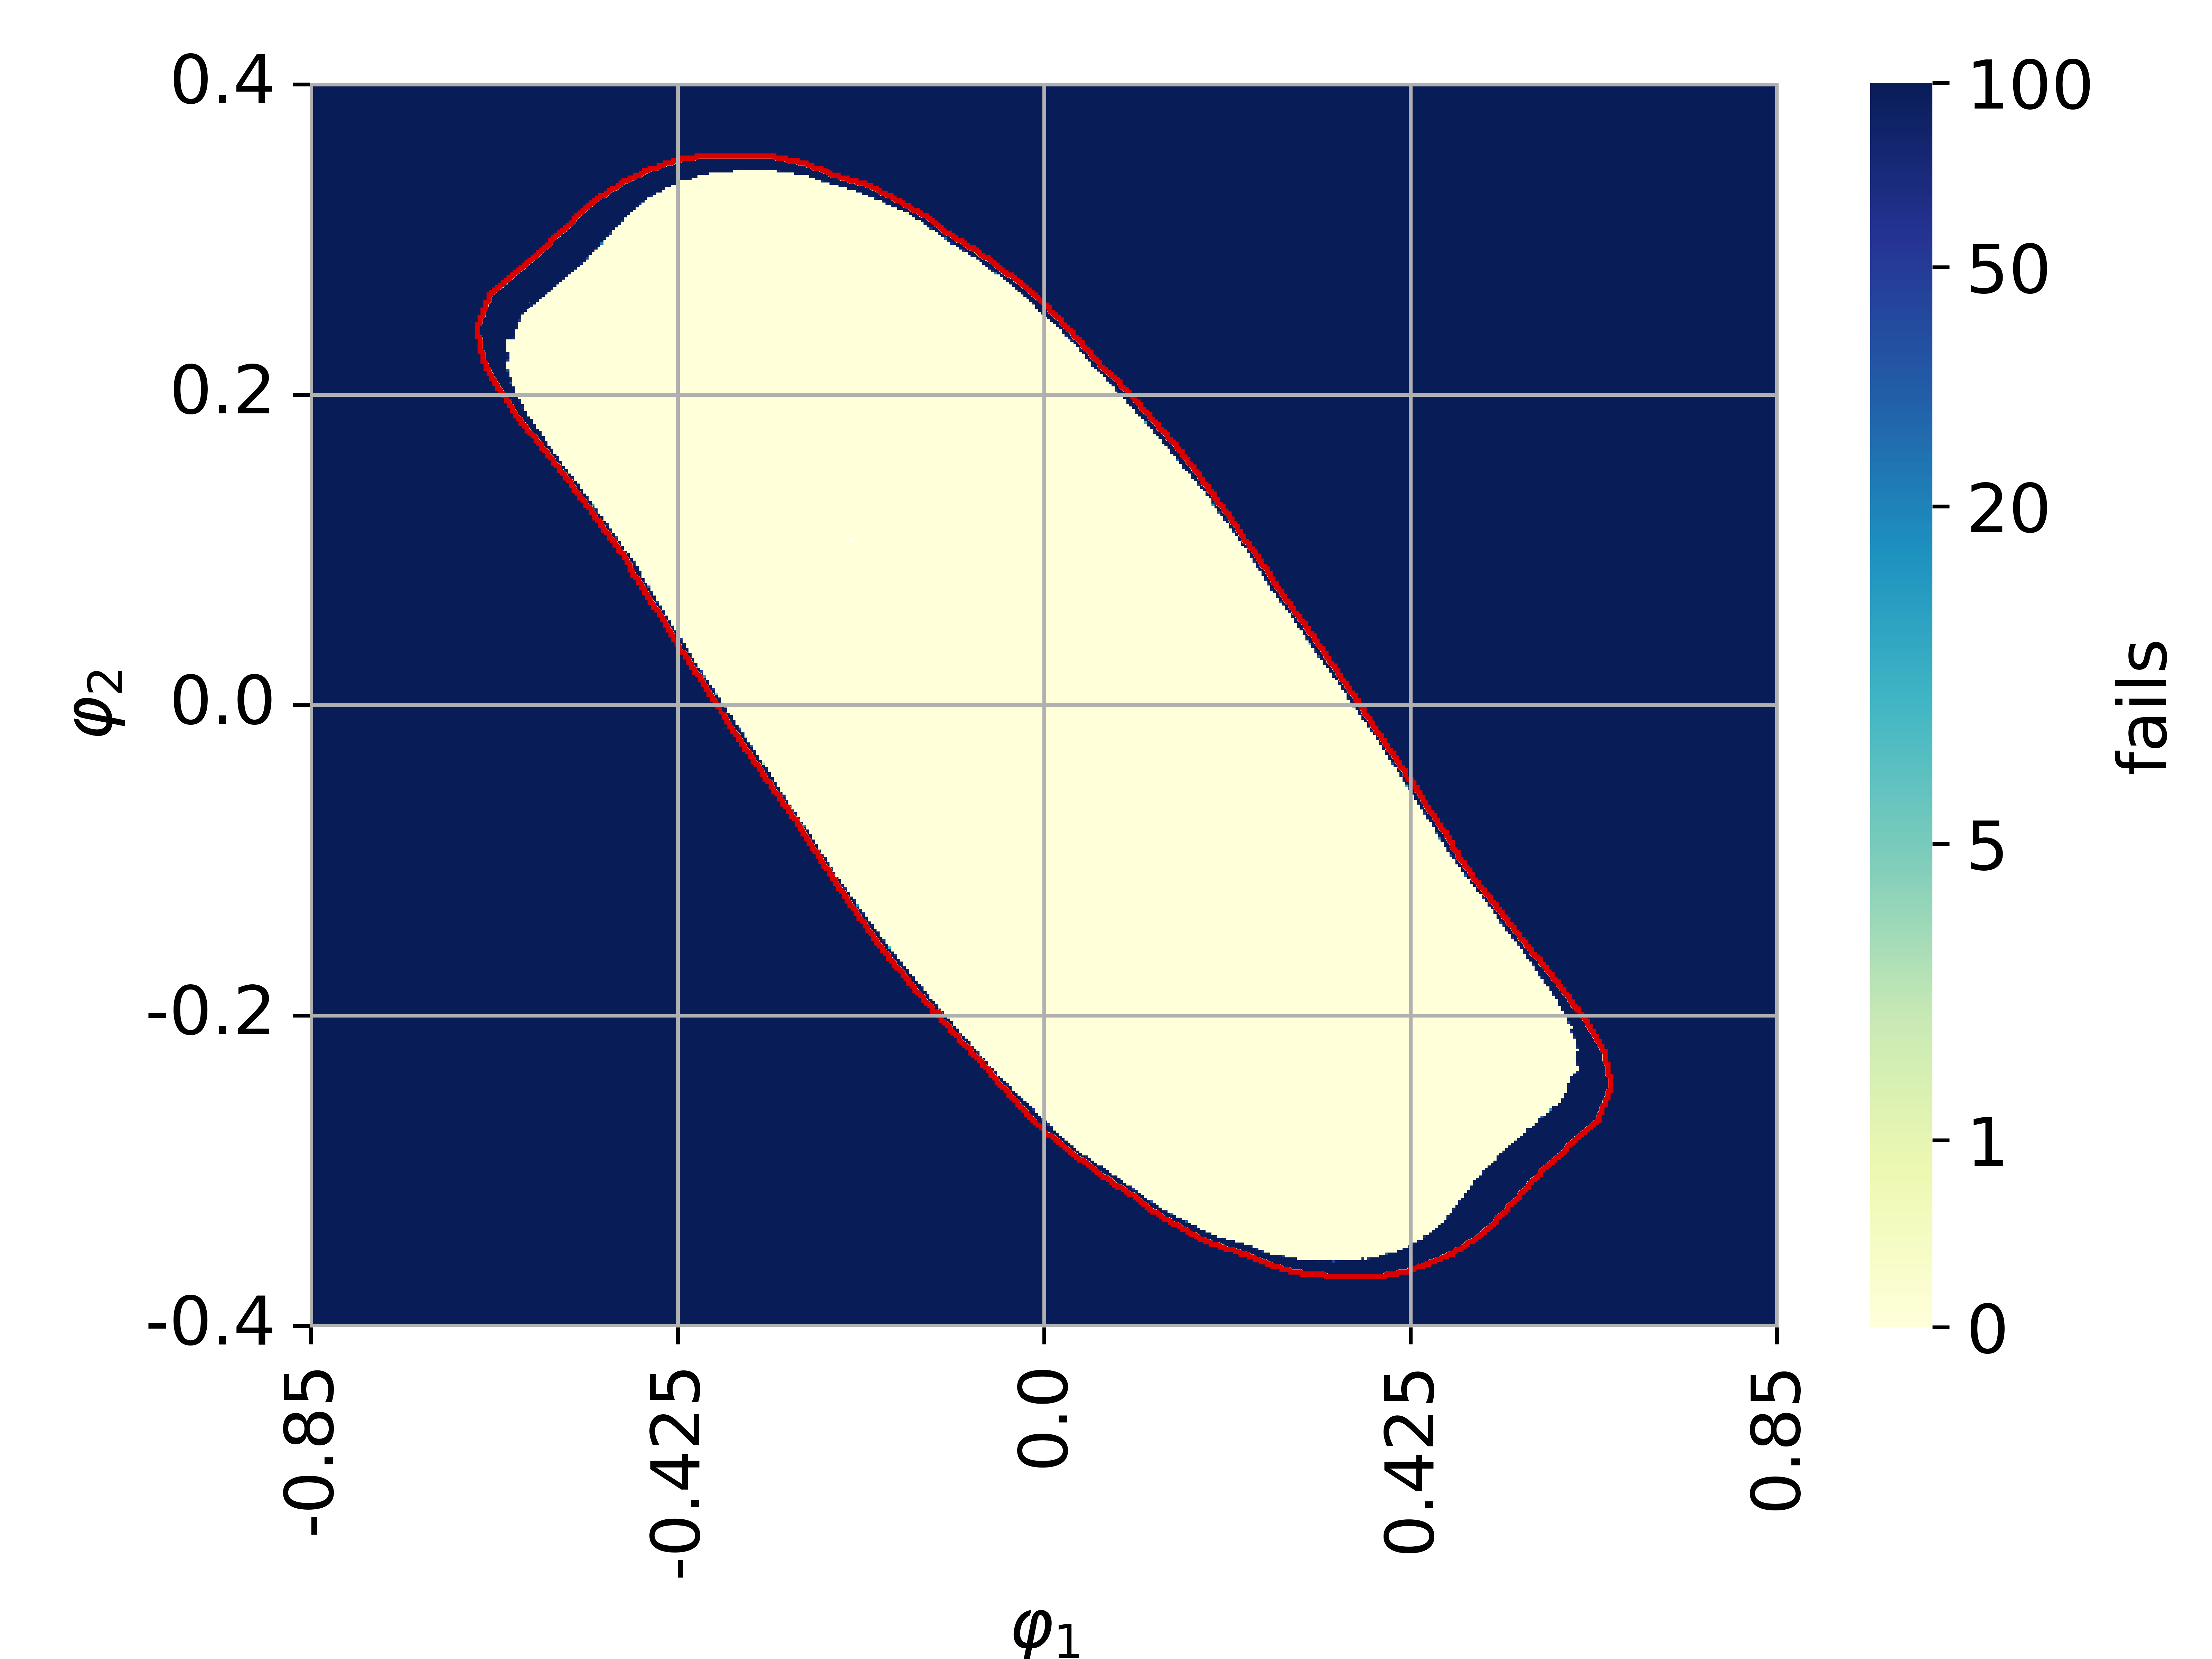
\includegraphics[width=\textwidth]{Figures/DP_friction_0.02.png}
         \label{fig: DP friction 0.02}
         \caption{}
     \end{subfigure}

     \caption{The stability zone for the double link system using the PPO agent, case 0. The red boundary corresponds to that depicted continuous control stability zone in Figure~\ref{fig: continuous vs discrete} (b). The environment parameters are modified as follows: (a) 1.1~$l$, (b) 1.2~$l$, (c) 1.1~$m$, (d) 1.2~$m$, (e) $f_{rel}$ = 0.01, and (f) $f_{rel}$ = 0.02.}
     \label{fig: agent impact on different environments}
 \end{figure}

The observations shows, that increasing the link length will cause the stability zone to expand (see Figures~\ref{fig: agent impact on different environments} (a) and (b)), while not having the increase of the blind spots, as it was for the discrete control cases~\cite{manzl2023relrl}. Increasing the mass of the link doesn't provide any differences from the base model (Figures~\ref{fig: agent impact on different environments} (c) and (d)), so that we can state that up to the changes of 20\% the model is independent from the link mass change, showing the same behavior as for the discrete model, where the changing of mass was also neglectable on the stability zones.
Considering friction the stability zone becomes smaller within each increase of it, but the value of \( f_{\text{rel}} = 0.02 \) still provides us with the stable zone without causing the agent to fail in the original contour (Figures~\ref{fig: agent impact on different environments} (e) and (f)), as it was shown in~\cite{manzl2023relrl}. It can be concluded that the continuous control scheme is more suitable if friction is involved in the environment model simulation.

\subsection{RL training enhancement with CL} \label{subsec: RL training enhancement with CL}

Before conducting the analysis there is a need to come up with baseline results of the continuous RL method PPO without its enhancement with Curriculum Learning. For this we have conducted tests using the system parameters presented in the Table~\ref{tab:hyperparameters} and~\ref{tab:env_params} for systems with 1 to 3 links. For each system there are 10 cases, which represent random initial states are simulated to show the variability of control across different initial conditions. The baseline is set according to the values of mean, median, minimum and maximum of training timesteps across cases, where mean and median are the main indicators to orient on. The Table~\ref{tab: baseline statistics for PPO in continuous action space} shows the results of the RL training using PPO algorithm in continuous action space.

\begin{table}[ht]
	\centering
	\caption{Baseline results of using PPO algorithm in continuous action space for 1 to 3 link pendulum systems}
	\begin{tabular}{@{}lccccc@{}}
		\toprule
		\textbf{System} & \textbf{Successful cases} & \textbf{Mean} & \textbf{Median} & \textbf{Minimum} & \textbf{Maximum} \\ \midrule
		\textit{1-link} & 10 & 26168 & 25600 & 24320 & 32000 \\
		\textit{2-link} & 7 & 48055 & 49152 & 38400 & 55296 \\
		\textit{3-link} & 5 & 278937 & 288768 & 194560 & 319488 \\ \bottomrule
	\end{tabular}
	\label{tab: baseline statistics for PPO in continuous action space}
\end{table}

To select the parameters needed for the CL implementation the research was conducted in steps. At first, we determine which decay type is specifically the most performing for our particular task of pendulum stabilization. For this we have simulated 150 runs of 5 cases within the control values matrix of the form 
\(\begin{bmatrix} 1 & n \\ 0 & 0 \end{bmatrix}\), where \(n = 2, 4, 6, 8, 10\) and decay steps vector \(\begin{bmatrix} 0 \\ k \end{bmatrix}\), where \(k = 5000, 6000, \ldots, 10000\) to evaluate the performance across different control parameters. The results are presented in a form of a bar plot, which shows the number of agent successes for the whole dataset. It is shown, that the exponential decay type function, provides the best results of having 74$\%$ of successes across the dataset. 

\begin{figure}[h]
	\centering
	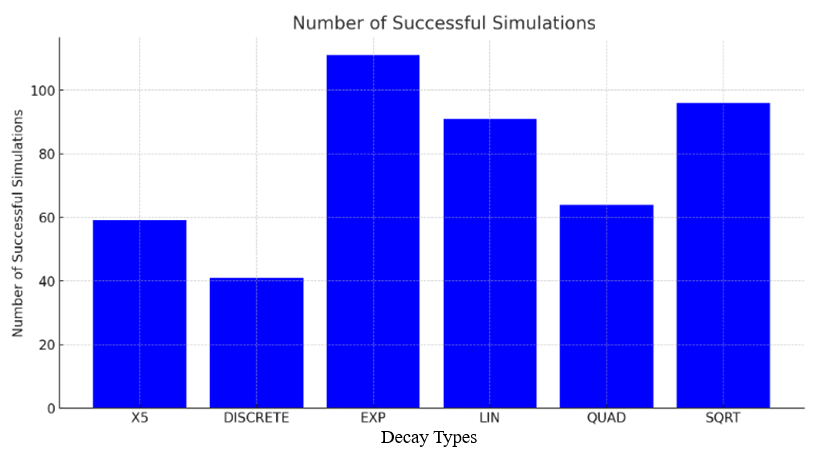
\includegraphics[width=10cm]{Figures/decay_types_results_comparison.png}
	\caption{}
	\label{fig: decay types comparison}
\end{figure}

Within the results of this research, later on we use exponential decay type to work with for the CL implementation. Next step includes the development of control values decay scheme to analyze their influence while varying decay steps.
% btw i have completely forgot about decay factor (should we add some simple description for it about why we have chosen 0.005?). Since i have the results on varying it on 5 different values, we can as well show some statistics here about it.
% can also be shown as a table, possible to say that our analysis was total: [1 n], [1 n n] and [1 n n n n] and that we have selected the best results out of those schemes)
% should we add comparison of decay factors?  
%\begin{table}[ht]
%	\centering
%	\caption{CL schemes for each pendulum system type}
%	\begin{tabular}{@{}lcc@{}}
%		\toprule
%		\textbf{System} & \textbf{Control values scheme} & \textbf{Decay steps} \\ \midrule
%		\textit{1-link} & \(\begin{bmatrix} 1 & n \\ 0 & 0 \end{bmatrix}\) & 1000 ... 12000, h = 1000 \\
%		\textit{2-link} & \(\begin{bmatrix} 1 & n & n \\ 0 & 0 & 0 \end{bmatrix}\) & 9000 ... 22000, h = 1000 \\
%		\textit{3-link} & \(\begin{bmatrix} 1 & n & n & n \\ 0 & 0 & 0 & 0 \end{bmatrix}\) & 30000 ... 50000, h = 1000 \\ \bottomrule
%	\end{tabular}
%	\label{tab: CL simulation data}
%\end{table}

For the single pendulum system the control values matrix is remained unchanged in the form of \(\begin{bmatrix} 1 & n \\ 0 & 0 \end{bmatrix}\), since the system is relatively simple and does not need a lot of restriction in its movements to improve the training speed. Experiments were conducted with $n$ value varying from 0.1 to 1 with step size equal to 0.1 and from 1 to 12 with step size equal to 1. Decay steps were varied from 1000 to 12000 with the step size of 1000. Double pendulum system control scheme is selected as \(\begin{bmatrix} 1 & c \cdot n & r \cdot n \\ 0 & 0 & 0 \end{bmatrix}\), where $c$ and $r$ are extension coefficients, implemented to see the difference in results, while varying the pendulum link constraints magnitude, where \(c = 1, 2, 4, 8\) and \(r = 1, 2, 4, 8\), while \(n = 1, 2, \ldots, 10\). Decay steps are varied from 9000 to 22000 with step size equal to 1000. For the triple link system the scheme \(\begin{bmatrix} 1 & 4n & 2n & n \\ 0 & 0 & 0 & 0 \end{bmatrix}\), where \(n = 1, 2, \ldots, 10\) is selected due to the need of stronger restriction on the first link, since it holds the mass of two attached to it next links. Variation of decay steps is performed from 30000 to 50000 with the step size equal to 1000. 
Evaluation of the obtained results is performed across cases within each distinctive combination of control values and decay steps and not across the whole control scheme, since the implemented Curriculum Learning requires these values, with which the controlled system can be trained faster and be more robust. To find the best combination of control values scheme and decay steps we focus on 3 main factors: number of successfully trained cases in each combination, mean and median values of the training time. For the single and double pendulum systems the successful case is the one which reaches 50/50 tests. For the triple pendulum system we were not able to reach an exact number of 100 successful tests, so the baseline of success is set to at least 70/100 tests being passed by the simulated system. The results are shown in the Table~\ref{tab: CL results}.

\begin{table}[ht]
	\centering
	\caption{CL enhancement: best results for 1 to 3 link pendulum systems}
	\begin{tabular}{@{}lccccc@{}}
		\toprule
		\textbf{System} & \makecell{\textbf{Best performing}\\ \textbf{schemes}} & \makecell{\textbf{Successful}\\ \textbf{cases}} & \makecell{\textbf{Decay}\\ \textbf{steps}} & \textbf{Mean} & \textbf{Median} \\ \midrule
		\textit{1-link} & \(\begin{bmatrix} 1 & 0.8 \\ 0 & 0 \end{bmatrix}\) & 10 & 7000 & 17817 & 18432 \\ \midrule
		\textit{2-link} & \(\begin{bmatrix} 1 & 20 & 5 \\ 0 & 0 & 0 \end{bmatrix}\) & 10 & 15000 & 43929 & 43008 \\ \midrule
		\textit{3-link} & \(\begin{bmatrix} 1 & 16 & 8 & 4 \\ 0 & 0 & 0 & 0 \end{bmatrix}\) & 10 & 30000 & 233676 & 216064 \\ \bottomrule
	\end{tabular}
	\label{tab: CL results}
\end{table}

According to the obtained results we are able to conclude, that for all 3 systems we have achieved an improvement in the amount of successfully trained cases (what means that the control became more robust) as well as in training time. The Table~\ref{tab: CL improvement statistics} shows the improvement of the training time in percents in accordance to our predetermined baseline. 

\begin{table}[ht]
	\centering
	\caption{Improvement statistics by enhancing RL training of the 1 to 3 link pendulum systems with CL}
	\begin{tabular}{@{}lcc@{}}
		\toprule
		\textbf{System} & \makecell{\textbf{Mean}\\ \textbf{improvement}} & \makecell{\textbf{Median}\\ \textbf{improvement}} \\ \midrule
		\textit{1-link} & 32\% & 28\% \\
		\textit{2-link} & 8.6\% & 12.5\% \\
		\textit{3-link} & 19\% & 25.2\% \\ \bottomrule
	\end{tabular}
	\label{tab: CL improvement statistics}
\end{table}
% results are open for improvements discussion
Overall, these results demonstrate a clear trend: as the complexity of the system increases, the effectiveness of Curriculum Learning in improving RL performance may decrease. While CL significantly enhances training for simpler systems, its impact diminishes for more complex, multi-link systems, where the RL agent faces greater challenges in learning and generalization. The relatively consistent performance for the 1-link system suggests that simpler systems benefit more uniformly from CL, while the larger discrepancies observed in the 2-link and 3-link systems indicate that more complex dynamics introduce greater variability in the training process. These findings highlight the importance of considering system complexity when designing RL curriculum and suggest that additional modifications to the curriculum strategy, such as dynamic adjustment based on the agent's performance, may be required to further improve learning outcomes for more complex systems.
% there can be a talk about that the main problem is actually searching for the best parameters if we really want to enhance our results, especially if talking about particular cases!